\documentclass{article}

% Pass numbered, compressed citations to natbib
\PassOptionsToPackage{numbers, sort&compress}{natbib}
% before loading neurips_2026

\usepackage[preprint]{neurips_2026}
% Options:
%  \usepackage[main]{neurips_2026}          % Main Track (double-blind)
%  \usepackage[preprint]{neurips_2026}      % arXiv / preprint
%  \usepackage[main, final]{neurips_2026}   % Camera-ready

\usepackage[utf8]{inputenc} % allow utf-8 input
\usepackage[T1]{fontenc}    % use 8-bit T1 fonts
\usepackage[colorlinks=true,linkcolor={blue!70!black},citecolor={blue!70!black},urlcolor={blue!70!black},hypertexnames=false]{hyperref}
\usepackage{url}            % simple URL typesetting
\usepackage{booktabs}       % professional-quality tables
\usepackage{colortbl}       % \cellcolor in tables
\usepackage{amsfonts}       % blackboard math symbols
\usepackage{nicefrac}       % compact symbols for 1/2, etc.
\usepackage{microtype}      % microtypography
\usepackage{xcolor}         % colors
\usepackage{graphicx}       % includegraphics
\usepackage{subcaption}     % subfigures with (a), (b) labels
\usepackage{amsmath,amssymb,amsthm} % math
\usepackage{algorithm}
\usepackage{algorithmic}
\usepackage[section]{placeins}
\usepackage{tikz}
\usetikzlibrary{arrows.meta,positioning,calc,decorations.pathreplacing,fit}

% Colors for agent states (Wong colorblind-safe palette)
\definecolor{buyblue}{HTML}{0072B2}
\definecolor{holdgray}{HTML}{AAAAAA}
\definecolor{sellorange}{HTML}{D55E00}
\definecolor{edgegreen}{HTML}{009E73}
\definecolor{lightbg}{HTML}{F0F0F0}
\definecolor{hlyellow}{HTML}{F0E442}

\setcounter{topnumber}{2}
\setcounter{bottomnumber}{1}
\renewcommand{\topfraction}{0.85}
\renewcommand{\bottomfraction}{0.85}
\renewcommand{\textfraction}{0.10}
\renewcommand{\floatpagefraction}{0.75}

\newtheorem{theorem}{Theorem}
\newtheorem{lemma}[theorem]{Lemma}
\newtheorem{proposition}[theorem]{Proposition}
\newtheorem{corollary}[theorem]{Corollary}
\theoremstyle{definition}
\newtheorem{definition}[theorem]{Definition}
\theoremstyle{remark}
\newtheorem{remark}[theorem]{Remark}

\title{Local rule activation and dealer capacity in a cellular automaton market\thanks{Repository: \url{https://github.com/varnerlab/Wolfram-markets-abm-paper.git}.}}

\hypersetup{
  pdftitle={Local rule activation and dealer capacity in a cellular automaton market},
  pdfauthor={Jeffrey D. Varner}
}

\author{%
  Jeffrey D. Varner \\
  R.F. Smith School of Chemical and Biomolecular Engineering\\
  Cornell University, Ithaca, NY 14850 \\
  \texttt{jdv27@cornell.edu} \\
}

\begin{document}
\raggedbottom
% Keep paragraph openings and endings together across page and display breaks.
\clubpenalty=10000
\widowpenalty=10000
\displaywidowpenalty=10000

\maketitle

\begin{abstract}
Changes in investor decisions can spread through a market, but the resulting
price decline depends on how trades execute. We developed a market model
in which traders inside a grid decided whether to buy, hold, or sell from
their neighbors' decisions, while technical traders at selected perimeter
sites responded to price. Paired markets shared the same history before
selected traders in one market received a persistent change in their
local decision rule. The comparison market retained its original rule.
A majority decided to sell when enough traders received the new response,
even though the remaining traders kept their original rules. Holding the
technical traders prevented price changes from entering later decisions,
yet majorities still formed, establishing that neighbor responses could
produce widespread selling. Comparisons across market sizes and observation
periods located a finite-time crossover whose position continued to depend
on the time observed. To connect decisions to prices, we cleared unit
orders against a dealer whose finite cash and share reserves retained a
constant product. The batch execution price and resulting marginal quote
were both determined by those reserves, preventing an isolated round trip
that restored dealer inventory from extracting its cash. Shallow positive
reserves accompanied severe declines while rejecting few orders backed by
trader resources. Zero reserves instead permitted only opposing trader
orders at a fixed price. Shallow markets also had large drawdowns without
the rule switch, making matched financial comparisons necessary for
attribution. Changing trader cash and shares affected interior decisions
only when technical traders could respond to the resulting prices.
The model separated the spread of selling decisions from the severity of
a simulated crash. Limited trading resources did not generally protect
against severe declines, because their financial consequences depended on
the mechanism linking execution to price.
\end{abstract}

% introduction.tex -- Introduction
\section{Introduction}

During the October 1987 market decline, portfolio insurance concentrated
selling across participating traders~\cite{shiller1988portfolio,grossman1988analysis}.
Forced sales by funds that had borrowed to invest spread losses across
quantitative equity strategies in August 2007~\cite{khandani2011what}.
Such episodes motivate a common modeling question: how can changes in
some investors' decision rules destabilize a market and contribute to
a crash? Agent-based
models address collective behavior through imitation, strategy adaptation,
and responses to a shared price~\cite{lebaron2006agent,hommes2006heterogeneous,samanidou2007agent,axtell2025agent}.
In the minority game, every trader reads the same record of past outcomes
and switches among strategies scored on that record, so traders interact
only through the market outcome~\cite{challet1997minority,challet2000modeling}.
In the Santa Fe artificial stock market, traders learn forecasting rules
from a shared price and dividend~\cite{lebaron1999time}; adding technical
rules to a trader's repertoire was a dominant strategy that lowered wealth
and raised volatility for all~\cite{joshi1999technical,joshi2002financial},
and how much technical trading emerged depended on details of the learning
algorithm~\cite{ehrentreich2006technical}.
Many of these models include technical traders, who decide from the recent
history of the price, alongside traders who follow fundamental value or the
opinions of others~\cite{brock1998heterogeneous,lux1999scaling,hommes2006heterogeneous}.
Herding models describe how individual decisions produce collective
activity~\cite{kirman1993ants,cont2000herd,lux1999scaling}, while lattice
models encode local interactions through stochastic imitation or spin-like
responses, sometimes alongside market-wide
signals~\cite{bornholdt2001ising,iori2002microsimulation,bartolozzi2004stochastic,qiu2007cellular,sornette2006importance}.
These interactions can generate large fluctuations and periods of sustained
volatility, two features of financial returns~\cite{cont2001empirical}.
These approaches explain fluctuations through several forms of interaction,
but their aggregate return statistics do not by themselves separate the
effects of a persistent local rule change from feedback through price.
Both the size of the changed group and the nature of the change matter. A temporary increase in selling
and a persistent change in how traders respond to their neighbors need
not produce the same collective outcome.

A cellular automaton represents investors as traders arranged on a square
grid, with each trader deciding whether to buy, hold, or sell from the
decisions of nearby traders. Each trader uses a lookup table to convert the
sum of its four neighbors' numbered decisions into its next decision, a
totalistic rule~\cite{wolfram1984universality,packard1985two,wolfram2002new}.
Wolfram's own market model placed buying and selling entities on a line,
each responding to its two neighbors under a fixed rule, and took the
running difference between buyers and sellers as the
price~\cite{wolfram2002new}. A recent model in which thirty-two agents
followed rules inspired by Rule~110, kept balance sheets, and set the price
from the counts of buy and sell positions produced series with the
statistics of real assets~\cite{valsan2022on}. Two-dimensional
cellular-automaton markets have instead used stochastic rules, typically a
probability that a trader imitates its neighbors, and varied that
probability or a market-wide factor to change market
behavior~\cite{wei2003cellular,bartolozzi2004stochastic,qiu2007cellular,fan2009effect,atman2012influence}.
The model studied here uses a deterministic table drawn from the complete
set of totalistic rules, so one table entry can change while the other
responses stay fixed. Asking a trader to sell once changes its current decision, whereas
changing the rule changes how it responds whenever the same neighbor sum
occurs again. The new rule remains in use even after the trader stops
selling. Starting two markets from the same history, then changing the rule
in only one, allows the effect of that change to be measured against
continued use of the original
rule~\cite{glasserman1992guidelines,law2015simulation}.
In this model, selected traders along the edge of the grid are
technical traders: they buy when the price falls below a band around its
recent average and sell when it rises above that band, and they are the only
traders whose decisions depend on the price. The question is how
many traders must receive the new rule before at least half of the interior
traders decide to sell, which we call a Sell majority, and whether this
instability can develop when the technical traders are kept in Hold, so that
trades still complete and the price still moves, but no decision responds to
it.

A market dominated by sellers and a market price crash are different
outcomes. Their connection depends partly on the resources needed to trade. A trader needs shares to sell or cash to
buy, and completing a trade requires someone willing and able to take the
other side. Dealers can complete orders that other traders do not match, but
their cash and share holdings limit how much they can buy and
sell~\cite{garman1976market,stoll1978supply,ho1981optimal,madhavan2000market,adrian2017dealer}.
Price-impact models describe how completed trades change the
price~\cite{kyle1985continuous,hasbrouck1991measuring,farmer2005predictive,bouchaud2009how}.
Agent-based markets have included limited trader resources, records of
outstanding buy and sell orders, borrowing limits, and dealers with limited
cash and
shares~\cite{raberto2001agent,chiarella2002simulation,thurner2012leverage,braunmunzinger2018agent}.
In the grid model, traders can keep deciding to sell even when they cannot
complete a sale, allowing instability in decisions to develop without a
price crash. Limits on completed trades also change the price that informs later decisions. Dealer capacity can therefore affect both selling decisions and prices. We coupled execution and price through a dealer whose finite cash and
share reserves retained a constant product, following the reserve-based
approach of constant-function markets~\cite{angeris2022constant}.
Each batch used a common execution price consistent with its net trade,
and the final reserve ratio set the next marginal quote. This construction
tied price movements to actual transfers and prevented an isolated round
trip that restored dealer inventory from extracting its cash. It also
made reserve depth determine both available funding and price sensitivity,
so a smaller dealer need not protect the market from a large decline.
The relevant comparison was how a given pattern of decisions traded
against different reserves, and how the resulting prices influenced
later decisions.

In this study, we used a three-state cellular automaton market to examine
how changes in investor decision rules produced market instability and
how trading resources connected those decisions to price declines.
We compared markets with a common history, then changed one response in
the lookup table of selected interior traders while preserving the
comparison market's rule. Keeping technical traders in Hold allowed the
same intervention to be studied without feedback from price, while still
calculating trades and financial outcomes. A one-time instruction to sell
and a screen of other single-response changes tested which features of
the intervention mattered. Comparisons across grid sizes and observation
periods assessed whether the fraction needed for a Sell majority depended
on the extent and duration of interaction. We also varied dealer reserves
and changed trader cash and shares separately to identify their effects
on completed orders, majority formation, and drawdown. The paired design
therefore addressed two linked questions: whether a persistent change in
local decisions could spread through neighboring traders, and how the
execution mechanism determined the accompanying price decline.


% methods.tex -- Methods
\section{Methods}

\subsection{Three-state cellular automaton}

We represented investors on an $L\times L$ square lattice. Traders
inside the lattice decided whether to buy, hold,
or sell by observing their immediate neighbors' decisions. On the other hand, selected traders
along the edge of the lattice were technical traders, who decided to buy, sell or hold
from the observed price alone:
each bought when the price fell below a band around its recent average and
sold when the price rose above that band. Completed trades used a common
execution price, but only the technical traders used the observed quote to
decide whether to buy, hold, or sell. Buy ($s=0$), Hold ($s=1$), and Sell
($s=2$) represented the resulting decisions, and the local rule specified
which decision a trader made for a given neighbor configuration. Only the $(L-2)^2$ interior
cells followed the cellular-automaton rule. All interior traders updated together from their four nearest
neighbors, denoted by $\partial i$. The input decisions $s_j^{\rm in}(t)$
were the previous interior decisions and the newly updated perimeter
decisions. Adding these inputs gave the sum $c_i(t)$. A lookup table ${\cal R}$ assigned
one next decision $a_j={\cal R}(j)$ to each possible sum.
The sum ranks Buy below Hold and Sell but does not distinguish all
combinations of neighboring decisions. Two Holds and two
Buys receive the same response as one Sell and three Buys.
Changing one table entry therefore altered the response to a specified
neighbor sum while preserving the other eight responses. Neighborhoods
with the same sum remained equivalent under the altered rule.
The local input and the Wolfram index $R$ encoding the nine
outputs were defined by the expressions~\cite{wolfram1984universality,packard1985two}:
\begin{gather}
  c_i(t)=\sum_{j\in\partial i}s_j^{\rm in}(t)\in\{0,1,\ldots,8\},
  \label{eq:neighborhood-sum}\\
  R=\sum_{j=0}^{8}a_j3^j.
  \label{eq:rule-index}
\end{gather}

Rule~19280, $(222110002)_3$, supplied the baseline decision rule.
The activated Rule~19286, $(222110022)_3$, differed only at $c=1$
(Eqs.~\ref{eq:neighborhood-sum} and~\ref{eq:rule-index}).
A neighborhood containing three Buys and one Hold therefore returned Buy
under the baseline and Sell under activation. Before each run, we selected
$\operatorname{round}(f(L-2)^2)$ interior sites uniformly without replacement
as the target set for the later switch. The reported fraction $f$ was
nominal; its realized value followed this integer rounding. The initial interior contained
$\operatorname{round}(0.05(L-2)^2)$ Buy sites and the same number of Sell
sites, with Hold elsewhere. Initial states were placed without replacement.
A random-number seed identified each starting market and fixed the
initial placements, selected traders, technical traders, and their
band parameters. It also fixed the priorities used
when eligible orders exceeded dealer capacity. Once these choices were
made, the market evolved deterministically. Delaying activation allowed
the market to develop under the baseline rule before the response changed.
At the intervention, each targeted trader retained its current decision
and holdings but used the new rule to make subsequent decisions. Traders
outside the target set kept their original decision rule throughout.

\subsection{Orders, trader resources, and completed trades}

A trader's decision generated a desired order, but completing it required
cash or shares and a counterparty. Every interior trader and technical
trader held cash $w_i$, an integer number of shares $q_i$, and average
purchase price $\bar c_i$. Buy requested one share, Sell offered one share,
and Hold requested no trade. All completed orders in a step used one
execution price, determined together with the quantities that could
trade. A buy was eligible only if the trader could pay that execution
price, and a sell required at least one share. The main experiments
disabled the optional restriction on selling below average acquisition
cost~\cite{shefrin1985disposition,odean1998investors}. We recorded desired
orders lacking trader resources as \emph{agent suppression}. A trader's
stored decision persisted even if its order failed: a trader could remain
in Sell without shares, and its neighbors still responded to that state.
Thus financial resources constrained execution without directly changing
the interior decision rule.

The dealer supplied unmatched orders from finite cash and share reserves.
Capacity $h$ specified initial dealer shares per trader. For $N_{\rm tr}$
traders and initial price $P_0=100$, the dealer started with
$H=\operatorname{round}(hN_{\rm tr})$ shares and cash $P_0H$.
For positive $h$, its cash $W$ and shares $Q$ followed a constant-product
reserve curve, a two-asset instance of constant-function market
making~\cite{angeris2022constant}. The dealer could neither borrow cash
nor sell borrowed shares, and retained at least one share. For a candidate
net purchase $x$ by traders, positive for purchases from the dealer and
negative for sales to it, the uniform execution price $F_t(x)$ was the
cash transfer per net share needed to preserve their product $K$:
\begin{gather}
 K=W_{t-1}Q_{t-1},\qquad Q_{t-1}-x\geq1,\notag\\
 F_t(x)=\frac{W_{t-1}}{Q_{t-1}-x}.
 \label{eq:execution-price}
\end{gather}
At this candidate price, $B_t(x)$ counted desired buys backed by enough
cash and $S_t(x)$ counted desired sells backed by shares. Their difference
at $x=0$ determined direction $d_t$. For nonzero direction we selected
the largest supported integer quantity, denoting the eligible counts at the
selected price by $B_t$ and $S_t$. The selected net purchase was $x_t$,
and $n_t^B$ and $n_t^S$ denoted executed trader buys and sells:
\begin{gather}
 d_t=\operatorname{sign}\{B_t(0)-S_t(0)\},\notag\\
 x_t=d_t\max\left\{k\in\mathbb{Z}_{\geq0}:
 Q_{t-1}-d_tk\geq1,\quad
 d_t[B_t(d_tk)-S_t(d_tk)]\geq k\right\},
 \label{eq:dealer-buy-excess}\\
 n_t^B=\min\{B_t,S_t+x_t\},\qquad n_t^S=n_t^B-x_t.
 \label{eq:dealer-sell-excess}
\end{gather}
For $d_t=0$, we set $x_t=0$. The smaller eligible side completed every
order, and reproducible priorities selected orders on the larger side
when it could not be filled completely. We recorded eligible orders left
unfilled as \emph{dealer rejection}. Rejection could reflect the final
share constraint or the inability to support another indivisible share
at its required price; it did not require zero dealer cash.

All executed trader orders settled at $F_t=F_t(x_t)$, including trades
matched between traders. Settlement changed the dealer's books and its
next marginal quote $P_t$ according to:
\begin{gather}
 Q_t=Q_{t-1}-x_t,\qquad W_t=W_{t-1}+F_tx_t,
 \label{eq:dealer-ledger}\\
 P_t=\frac{W_t}{Q_t}
     =P_{t-1}\left(\frac{Q_{t-1}}{Q_{t-1}-x_t}\right)^2.
 \label{eq:price-update}
\end{gather}
The execution price and the resulting marginal quote therefore differed
when net dealer trading was nonzero. Cash and shares were conserved
across traders and dealer, except at scheduled changes in trader
resources. In exact arithmetic, $W_tQ_t=K$ made an isolated sequence
returning dealer inventory to its initial value return dealer cash as
well. Such a round trip could not extract cash from the dealer. This
identity concerns isolated net trades; it does not rule out gains from
other traders. We applied no additional exponential price adjustment.
Reserve depth consequently determined both funding and sensitivity of
price to net trades. The deep comparison used finite $h=100$ throughout.
At $h=0$, opposing trader orders matched at the unchanged quote, with
no net dealer trade. This separate case supplied a fixed-price control
(Algorithm~\ref{alg:dealer-clearing}).

\subsection{Technical traders and price feedback}

Selected traders along the edge of the grid brought price information
into neighboring decisions. They followed a rule of the Bollinger-band
type: each bought below a band around a recent price average, sold above
it, and held inside. This rule was contrarian, in contrast to the
trend-following moving-average rules often tested in market
data~\cite{brock1992simple}. One quarter of perimeter cells held technical
traders; the other perimeter cells stayed in Hold. A technical trader
compared the new marginal quote with reference price $\mu_t$ and a band
whose width used recent absolute price departures $\sigma_t$.
Each trader retained a multiplier $k_j\sim U[0.5,1.5]$, giving lower
and upper limits $\mu_t-k_j\sigma_t$ and $\mu_t+k_j\sigma_t$.
The normalized net purchase $\phi_t$ described completed orders but did
not separately set price. With smoothing parameter $\alpha=1/60$, the
recorded imbalance and updated band state were defined by:
\begin{gather}
 \phi_t=\frac{x_t}{N_{\rm tr}},
 \label{eq:imbalance}\\
 \mu_t=\mu_{t-1}+\alpha(P_t-\mu_{t-1}),\qquad
 \sigma_t=\sigma_{t-1}+\alpha(|P_t-\mu_t|-\sigma_{t-1}).
 \label{eq:adaptive-band}
\end{gather}

Orders came from the stored decisions at the start of each step.
Scheduled rule and resource changes preceded order collection, clearing,
and settlement. The new reserve ratio then set the marginal quote,
technical traders responded to it, and interior traders updated together
using old interior decisions and the new technical-trader decisions
(Algorithm~\ref{alg:model-step}). The complete step followed the sequence:
\begin{equation*}
 \text{stored decisions}\rightarrow\text{orders}\rightarrow\text{batch clearing}
 \rightarrow P_t\rightarrow\text{technical decisions}\rightarrow\text{interior update}.
\end{equation*}
We prevented price feedback by setting every technical trader to Hold
before each interior update. We call this condition \emph{technical
traders held}; \emph{technical traders active} denotes their response
to the new quote. Figure legends abbreviate these conditions as held
and active. The comparison retained the same initial grid, target set,
technical-trader locations and parameters, and financial resources.
Every held market still used the complete financial simulator. Cash,
shares, and price could change, but those changes could no longer
influence decisions inside the grid. Comparing held and active markets
therefore tested whether a Sell majority could develop from responses
to neighbors without feedback from prices.

\subsection{Paired rule-switch experiments}

We compared the consequences of changing a decision rule with continued
use of the original rule in paired markets that shared a common history. Both paths used Rule~19280 at every interior site for
$T_{\rm pre}=1{,}000$ baseline steps. At the start of step
$T_{\rm pre}+1$, one path activated Rule~19286 at the preselected fraction
$f$. The matched control left those sites on Rule~19280.
Neither path reset the lattice, price, technical traders' bands, trader holdings, or
dealer. Their common state $X_{T_{\rm pre}}$ also generated the first price
after activation, so the earliest possible difference occurred in the
following interior update. In the main paired rule-switch campaigns, we
checked the shared pre-switch histories and first post-switch price bit for bit.
Each switched path thus began with the same trader resources and
neighbor configurations as its control. The four main sets of simulations used 50 seeds and 3,000 steps after
the rule change, with initial trader cash of 1,000 and ten shares each. Additional comparisons tested other rules, a one-time instruction to
sell, fixed widths for the technical traders' bands, additional reserve depths, and longer observation periods.
The supplementary protocols specify which part of the intervention
or feedback was changed in each control (Appendix~\ref{app:revision-controls}).

We varied the fraction of traders given the new rule, grid size, and
financial resources to determine when a Sell majority formed and how
many sales could complete (Supplementary Table~\ref{tab:campaigns}).
The selected switch
experiment used $L=64$, a dealer with $h=100$, and active technical traders at
four activation fractions. We then tested more fractions at eight dealer capacities under both
technical-trader conditions. The finite-size campaign
used $L\in\{32,48,64,96,128\}$ with the technical traders held and $h=100$,
or active and $h\in\{1,100\}$. Because capacity was defined
per trader, absolute dealer resources increased with lattice size.
The financial campaign multiplied current trader cash and shares independently
by $g_w,g_q\in\{0.1,1,10\}$ at activation, rounding shares to integers.
Its nine interventions shared the same pre-intervention path within each
$(f,h,\text{technical traders},\text{seed})$ cell. With the technical traders held, they also
had to retain identical lattice trajectories afterward because neither cash nor shares entered the
interior update directly.
A discrepancy would therefore indicate an implementation error.
The appendix gives the full parameter grids and the checks used to verify
these paired relationships and the identities required when the technical
traders were held.

\subsection{Market outcomes, statistical analysis, and selection of examples}

We used the strictly interior Sell fraction $m(t)$ to measure the
shift toward selling. Larger values indicated that more interior
traders occupied Sell, and we treated the emergence of a Sell majority
after the rule change as a sign of market instability.
We recorded a Sell majority when $m(t)\geq0.5$ at least once after the
rule change. The onset time was the first step that reached this value,
and majority probability was the fraction of runs that reached it. We summarized onset times only for
runs that reached a majority and averaged the Sell fraction over the
final 500 steps to describe each market near the end of the observation
period.
To measure how much this final mean $\bar m$ differed between runs,
we multiplied its variance by the number of interior traders,
$(L-2)^2$, with angle brackets denoting averages across seeds. This
scaled variance is the susceptibility $\chi_L$, which allows comparison
across grid sizes~\cite{binder1981finite,landau2021guide}:
\begin{equation}
 \chi_L=(L-2)^2\left[\langle\bar m^2\rangle-
                         \langle\bar m\rangle^2\right].
 \label{eq:susceptibility}
\end{equation}
At a fixed grid size, higher susceptibility indicated greater
variation in the final mean Sell fraction between starting markets
(Eq.~\ref{eq:susceptibility}). Linear
interpolation gave $f_q(L)$, the activation fraction at which the
transition probability reached $q/100$. The midpoint was $f_{50}(L)$,
and the width $f_{75}(L)-f_{25}(L)$ measured how much additional
activation separated probabilities of 0.25 and 0.75. A smaller width
therefore indicated a sharper response.
Interpolation used the first upward crossing without forcing the sampled
curve to be monotone. Binomial proportions used 95\% Wilson
intervals~\cite{wilson1927probable}; continuous summaries used interquartile
ranges unless otherwise specified.

A high Sell fraction need not produce a large price decline if the
requested orders cannot execute. We measured the decline by maximum
drawdown, the largest proportional fall from a running price peak
during the post-activation window. We used price crash to describe a
large simulated decline and reported its magnitude through drawdown,
without defining a cutoff for classifying runs as crashes. We recorded unfilled orders at the
stage where resources prevented execution. Agent suppression counted
desired orders excluded by insufficient trader cash or shares.
Dealer rejection counted eligible orders left unfilled at the selected
execution price. In every campaign, the rejection fraction divided
post-activation rejected orders by post-activation eligible orders.
Agent suppression and completed-order counts used the same window.
The price window included the quote immediately before the rule change,
while majority detection began with the first updated interior state
after that change. Onset therefore began at step one; a missing onset
indicated no crossing within the observation period. Financial summaries used medians
and interquartile ranges across seeds. Drawdown measured the price decline caused by completed trades, while
suppression and rejection identified why desired trades could not
complete.

Testing too few fractions of traders with the new rule could miss the
range over which majority probability changed. We refined each curve using a common
resolution criterion. Intervals intersecting the empirical 5--95\% response were
bisected for up to ten rounds, aiming for at least five fractions
strictly inside that probability range in each size and condition.
Unbracketed crossings and unresolved curves remained explicitly missing
or flagged; observed outcomes were not used as pass conditions. Each added fraction used
the original 50 seeds. We then resampled whole seeds across all fractions
2,000 times to estimate uncertainty in the crossings, width, and sampled
susceptibility maximum. These percentile intervals preserved dependence
between fractions and included reselection of the susceptibility peak.
We also fitted a logistic curve, which required majority probability
$p_L(f)$ to increase smoothly with the fraction $f$. The fitted
parameters $a_L$ and $b_L$ controlled its position and slope:
\begin{equation*}
p_L(f)=\left\{1+\exp\left[-a_L-b_L(f-0.18)/0.01\right]\right\}^{-1},
\qquad b_L>0.
\end{equation*}
We fitted this curve by binomial likelihood and used the same seed blocks
to bootstrap its midpoint and width. Fitted standard errors were bootstrap
standard deviations. Both analyses measured uncertainty for the tested fractions and
observation period. Neither included error from interpolation, the
choice of additional fractions, or observing the market for longer.

We selected examples of traders' decisions across the grid using the
measured time to a majority or final Sell fraction to choose each run.
Selection preceded inspection of the images, with the smaller seed
breaking equal distances from a group median.
The newly computed 3,000-step results supplied a run without a majority at
$f=0.15$, both outcomes at $f=0.175$, and runs with a majority at
$f=0.185$ and 0.20 under $h=100$ (Fig.~\ref{fig:dose-panels}).
Among runs that reached a majority, we selected the run nearest the
group's median onset time. Among runs without a majority, we selected
the run nearest the group's median final Sell fraction. The dealer panels
required a single seed that transitioned at $h=0.1$, 1, and $100$ for
$f=0.20$. Among eligible seeds, selection minimized the summed distance
from the three capacity-specific median onsets. We extended the five examples
across fractions assigned the new rule to 10,000 steps after the change, with
snapshots at 0, 1,500, 3,000, 5,000, and 10,000 steps
(Fig.~\ref{fig:dose-panels}). The dealer comparisons retained their original
3,000-step duration and snapshots at 0, 500, 1,500, and 3,000 steps.
Selection therefore represented typical outcomes within each group over
the original observation period. A market without a majority at that
endpoint could reach one later. Individual runs illustrated how groups of
sellers developed, while
probabilities across runs measured how often a majority occurred.


% Generated by code/rebuild/WriteResults.py from corrected-run outputs.
\section{Results}

To explore how a persistent change in investor decisions could destabilize
a market, we changed one response in selected traders' rules and found
that a Sell majority formed when enough traders received the new rule
(Fig.~\ref{fig:rule-quench}; Supplementary Tables~\ref{tab:campaigns}
and~\ref{tab:paired-switch}).
Rule~19286 changed the response to three neighbors in Buy and one in Hold
from Buy to Sell, preserving every other response
(Fig.~\ref{fig:rule-quench}A,B). Each treated market shared its baseline
history and first post-switch quote with a comparison market that retained
Rule~19280. With active technical traders and dealer depth $h=100$, none
of the 50 starting markets reached a majority at $f=0.10$ or 0.15, whereas
all reached one at $f=0.20$ and 0.25. No matched control reached a majority
over the same period. The median onset among the two larger fractions
changed from 1,070.0 to 311.5
steps (Supplementary Table~\ref{tab:paired-switch}). In the selected
pair, groups of sellers expanded after the rule change while the
comparison market retained mixed decisions (Fig.~\ref{fig:rule-quench}C).
The lasting rule change also differed from a temporary instruction:
setting the selected traders to Sell once at $f=0.15$, 0.20, or 0.25
produced no majority in either technical-trader condition (Supplementary Table~\ref{tab:revision-pulse}).
Among the eighteen single-response rule changes tested at $f=0.20$,
6 produced a majority in every tested starting market under both feedback conditions, while 12 produced none (Supplementary Table~\ref{tab:revision-rules}).
Within these tested interventions, majority formation differed with the
changed response, the fraction of traders receiving it, and whether the
intervention changed a rule or only the current decision.

To determine whether price feedback was required for widespread selling,
we repeated the rule switch while keeping technical traders in Hold and
found that a majority still formed (Fig.~\ref{fig:reservoir}).
With these traders held, majority probability was 0.34
at $f=0.175$, 0.70 at $f=0.185$, and
1.00 at $f=0.20$ (Fig.~\ref{fig:reservoir}A).
Every held market was simulated again with its full cash, share, and price
history. Across dealer depths, onset, final mean Sell fraction, and final
interior states were identical for the same starting market and target
fraction, although the associated financial paths differed. This agreed
with the held update, which had no input from financial variables. Neighbor responses
were therefore sufficient to produce a Sell majority. Allowing
technical traders to respond to price changed majority frequency near
the crossover between mostly mixed and mostly Sell-majority outcomes.
At $h=100$, the active condition gave 25 of 50
majorities at $f=0.175$ and 42 at $f=0.185$,
compared with 17 and
35 when held (Fig.~\ref{fig:reservoir}A,B).
Both the size and direction of the active-minus-held difference depended
on the tested depth and fraction. A price response could thus modify
how often the rule change produced a majority, but it was not necessary
for selling decisions to spread. These comparisons separated the local
decision mechanism from feedback through completed trades.

To determine how the spread of selling depended on the number of
interacting traders, we compared grid sizes with technical traders held
and found a sharper majority response on larger grids
(Fig.~\ref{fig:finite-size}). We refined the fractions near each
response while retaining the same starting markets. At the original
3,000-step horizon, the interpolated fraction at which half the markets
reached a majority, $f_{50}$, changed from 0.216 at $L=32$ to
0.166 at $L=128$. The width separating majority probabilities
of 0.25 and 0.75 changed from 0.023 [0.018, 0.027] to
0.008 [0.004, 0.010], with brackets giving 95\% intervals from
resampling whole starting markets (Fig.~\ref{fig:finite-size}A,C;
Supplementary Table~\ref{tab:finite-size-scaling}). Variation in the
final mean Sell fraction also changed: its variance multiplied by the
number of interior traders, the susceptibility, had sampled maxima of
21.2 and 241.2 at the
endpoint sizes (Fig.~\ref{fig:finite-size}B,D). Across all size and
feedback conditions, the largest absolute difference between logistic
and interpolated midpoints was 0.0035, indicating the sensitivity
of the estimate to the imposed curve shape
(Supplementary Tables~\ref{tab:finite-size-scaling} and~\ref{tab:revision-fits}). Observation time
remained consequential. At $L=64$, extending the held markets from
3,000 to 9,000 steps changed the majority midpoint from
0.178 to 0.167; alternative
Sell thresholds and size-dependent horizons were measured separately
(Supplementary Table~\ref{tab:revision-horizons}). The size response
therefore described a crossover within the observation window, while
the continued movement with time prevented its interpretation as a
fixed threshold for indefinitely long runs.


To examine how the spatial patterns developed beyond the initial
observation window, we extended five numerically selected markets and
found that longer observation changed some outcomes
(Fig.~\ref{fig:dose-panels}). Selection used the newly computed
3,000-step results and preceded inspection of images. Two selected
markets had not reached a majority at that endpoint, while three had.
At 10,000 steps, 1 of the initially nonmajority examples had
crossed one-half. The first-majority outcomes, in displayed order, were
$f=0.150$, starting market 2: not within 10,000 steps; $f=0.175$, starting market 15: after 4{,}073 steps; $f=0.175$, starting market 41: after 2{,}330 steps; $f=0.185$, starting market 5: after 1{,}836 steps; $f=0.200$, starting market 38: after 1{,}028 steps (Supplementary Table~\ref{tab:market-panel-horizons}).
The spatial histories connected these crossings to the growth and
merger of groups of sellers, while the price histories measured their
financial consequences (Fig.~\ref{fig:dose-panels}A--C). In the selected
$f=0.175$ market that had not crossed by 3,000 steps, maximum drawdown
changed from 10.17\% to
26.34\% at the longer endpoint
(Supplementary Table~\ref{tab:market-panel-horizons}).
We also extended all 50 starting markets at $f=0.150$, retaining
matched no-switch comparisons. The number of majorities among changed-rule
markets was 0 at 3,000 steps and
2 at 10,000 steps,
while 0 controls reached a majority by
10,000 steps. Median drawdown changed from
5.04\% to 5.87\%,
and the largest observed drawdown changed from
12.29\% to 25.30\%
(Supplementary Table~\ref{tab:market-panel-horizons}).
The longer trajectories therefore qualified outcomes defined by the
original endpoint; persistence of mixed decisions over that shorter
window did not establish persistence over longer times.

We varied dealer depth while retaining the same decision-rule intervention
and found that shallower positive reserves accompanied larger price
declines, while majority probability did not vary monotonically with
depth (Fig.~\ref{fig:reservoir}). At $f=0.20$, every starting market
reached a majority at every tested depth. With active technical traders,
median maximum drawdown was 99.99\% at $h=0.1$,
99.52\% at $h=1$, and 25.15\% at $h=100$
(Fig.~\ref{fig:reservoir}C). The corresponding median rejection
fractions were 0.000226, 0.000034, and
0.0000006, so small positive reserves supported large declines
while rejecting few orders backed by trader resources
(Fig.~\ref{fig:reservoir}D). Zero depth supplied a separate limit:
only opposing trader orders matched, net dealer trading was zero, and
price stayed fixed. No-switch markets at $h=0.1$ already had median
drawdown 77.04\%, compared with
0.75\% at $h=100$. The median paired
increase after the rule switch was 22.96
percentage points at $h=0.1$ and 24.39
at $h=100$ (Supplementary Table~\ref{tab:paired-switch}).
Positive reserve depth changed both available
funding and the price required to execute a net trade. In the additional
comparison at $h=40$ and $h=400$, median drawdowns were
48.62\% and
7.08\%, respectively
(Supplementary Table~\ref{tab:revision-impact}).
Near the majority crossover, depth also changed feedback through the
technical traders. At $f=0.175$, majority probabilities were
0.44 at $h=0.1$ and 0.50 at $h=100$.
Their difference changed from -0.06 with
adaptive band widths to -0.26 with frozen widths
(Supplementary Table~\ref{tab:revision-band}). The paired difference
between those contrasts was 0.20, with a 95\%
bootstrap interval [-0.08, 0.50], so its sign was
not resolved (Supplementary Table~\ref{tab:revision-band}). The selected comparison
from starting market 2 also reached a majority at all three
displayed depths while following distinct price paths
(Fig.~\ref{fig:dealer-panels}). The reserve mechanism thus separated
majority formation from the severity of the decline, but shallow positive
reserves did not prevent severe drawdowns.

To distinguish trader resources from dealer reserves, we changed cash
and share holdings independently at the rule switch and found that
financial resources changed interior decisions only through active
price feedback (Fig.~\ref{fig:balance-sheet}). At $f=0.18$, all
cash and share combinations with technical traders held produced the
same decision history within a starting market, giving majority
probability 0.64 across dealer depths. With technical traders
active, probabilities ranged from 0.54
to 0.80
(Fig.~\ref{fig:balance-sheet}A; Supplementary Table~\ref{tab:balance-fractions}).
Holdings entered the order and clearing calculations but did not enter
the interior lookup table. Their effect on subsequent decisions therefore
required the intervening price response. With unchanged cash and $h=100$,
share multipliers 0.1, 1, and 10 gave median drawdowns of
3.17\%, 20.18\%, and 77.55\%,
respectively (Fig.~\ref{fig:balance-sheet}B). More shares supplied
more potential sales, while the reserve curve determined the price
at which net selling could clear. Increasing the cash multiplier from 1
to 10 at $h=1$ with unchanged shares changed median drawdown from 96.46\%
to 97.10\%, and majority probability from
0.58 to 0.56
(Fig.~\ref{fig:balance-sheet}A,B). Rejection recorded the fraction
of orders backed by trader resources that still failed to execute,
and its relationship to drawdown differed across the resource
combinations (Fig.~\ref{fig:balance-sheet}C,D). The financial
consequences of a rule change therefore depended on both sides of
traders' books and the dealer's reserves. A majority decision to sell
alone did not specify how many shares could change hands or how far
the marginal quote would fall.


% discussion.tex -- Discussion
\section{Discussion}

Changes in investor decision rules spread selling through the market,
while trader resources and the dealer's reserve curve determined the
associated price decline. A majority entered Sell after enough traders
received a new response to their neighbors, even though other traders
retained their original rules (Fig.~\ref{fig:rule-quench}). The changed
response remained available whenever the relevant neighbor configuration
recurred, rather than requiring selected traders to remain in Sell.
Comparing a persistent rule change with a one-time instruction to sell
separated this continuing influence from the immediate change in current
decisions (Supplementary Table~\ref{tab:revision-pulse}). The alternative
rule screen further tested which responses could produce a majority,
so the selected rule was examined within a defined set of local changes
rather than treated as a universal description of investor behavior
(Supplementary Table~\ref{tab:revision-rules}). The paired design made
the no-switch path the comparison for the intervention at each starting
market~\cite{glasserman1992guidelines,law2015simulation}. Repeating the
pair across starting markets then measured how frequently a majority
formed within the observation window. This interpretation concerned
assigned decision rules and their propagation through neighbors; traders
did not learn the new rule, choose it for its profitability, or pass
the rule itself to other traders.

The decision instability could develop without a price response entering
later decisions. Holding the technical traders removed that route of
influence, yet the rule change still produced Sell majorities
(Fig.~\ref{fig:reservoir}). In the spatial examples, growing groups of
sellers linked local responses to changes across the grid
(Fig.~\ref{fig:dose-panels}). Such patterns resemble the growth of
ordered regions in other interacting systems away from
equilibrium~\cite{hinrichsen2000nonequilibrium,bray1994theory}, while
dependence on the changed fraction connects the model to accounts of
how local changes spread through a
population~\cite{granovetter1978threshold,watts2002simple,aizenman1988metastability,holroyd2003sharp}.
The finite-size comparisons described a sharper majority response on
larger grids, but the estimated midpoint continued to depend on the
observation period (Fig.~\ref{fig:finite-size}; Supplementary
Table~\ref{tab:revision-horizons}). A market remaining mixed at one
endpoint could therefore require further observation before its later
outcome was known. Neither the selected images nor the sampled crossing
curves established a threshold for indefinitely large or long-lived
markets~\cite{binder1981finite,landau2021guide}. The resemblance to
droplets forming and joining also did not establish classical nucleation.
We measured no energy barrier, surface tension, formation rate, or
critical group size separating growth from decay. The supported
mechanism was the propagation of changed responses through neighboring
decisions over finite grids and observation windows.

The corrected execution mechanism changed the financial interpretation
of limited dealer resources. Dealer models commonly connect trading
to intermediary cash and inventory~\cite{garman1976market,stoll1978supply,ho1981optimal,braunmunzinger2018agent},
but holdings alone do not specify how those resources translate into
prices. Here, the constant-product reserve curve determined both the
uniform price that supported a batch and the marginal quote left after
settlement~\cite{angeris2022constant}. When the dealer bought shares,
its share reserve increased and its cash reserve decreased, so subsequent
net sales could execute at lower prices. Shallow positive reserves thus
allowed large proportional declines without requiring a large fraction
of eligible orders to be rejected (Fig.~\ref{fig:reservoir}C,D).
Zero depth was a separate fixed-price control, because the dealer took
no net position and only opposing trader orders matched. This distinction
prevented the zero-depth case from being read as evidence that every
small dealer protected the market from a crash. The no-switch comparisons
also mattered because shallow markets had large drawdowns while
retaining the original decision rule
(Supplementary Table~\ref{tab:paired-switch}). The paired increases
separated that baseline financial variation from the intervention.
The evidence therefore linked crash magnitude to the execution and
price mechanism as well as to available resources; resource scarcity
alone did not imply a small proportional decline.

Financial conditions could also feed back into the spread of selling.
Changing dealer depth or trader holdings altered completed orders and
prices, which then changed technical-trader decisions and the local
inputs seen by their neighbors (Figs.~\ref{fig:reservoir}
and~\ref{fig:balance-sheet}). Holding those traders prevented the same
financial changes from entering the interior update, providing an exact
control on this route of influence. With technical traders active,
majority probability did not consistently increase or decrease with
depth, even though drawdown at the comparison with $f=0.20$
decreased across positive depths. Freezing the Hold-band width tested
one contributor to feedback while preserving responses to a moving
reference price (Supplementary Table~\ref{tab:revision-band}). That
comparison did not remove technical trading, and its frozen widths
retained differences accumulated during each starting market's baseline.
The uncertainty in the paired contrast also prevented a clear attribution
of the depth difference to width adaptation.
The additional reserve-depth series changed funding and initial price
sensitivity together, so it could not identify their independent effects
(Supplementary Table~\ref{tab:revision-impact}). This coupling distinguishes
the experiment from models that assign a separate impact coefficient
to completed order imbalance~\cite{kyle1985continuous,farmer2005predictive,bouchaud2009how}.
Majority probability and drawdown consequently measured different
outcomes: the share of markets in which enough traders decided to sell,
and the size of the largest decline along the resulting price path.
Neither outcome alone specified the other.

The model differed from established agent-based markets in where traders
interacted and in what was changed. In the minority game, every trader reads
the same record of past outcomes, keeps a score for each of its strategies,
and uses the one that would have done best, so traders interact only through
the market outcome and the main control parameter is the number of
distinguishable histories relative to the number of
traders~\cite{challet1997minority,challet2000modeling}. In the Santa Fe
artificial stock market, traders learn forecasting rules from a shared price
and dividend~\cite{lebaron1999time}; adding technical rules to a trader's
repertoire was a dominant strategy that lowered wealth and raised volatility
for all~\cite{joshi1999technical}, and the rate at which traders revised
their rules settled at an equilibrium that left earnings below what slower
revision would have produced~\cite{joshi2002financial}. Models with
chartists and fundamentalists let traders move between the two groups at
rates set by recent profits or by the opinions of
others~\cite{lux1999scaling,brock1998heterogeneous,kirman1993ants}. Lattice
and cellular-automaton markets encoded local interactions through stochastic
imitation or spin-like responses, sometimes alongside market-wide
signals~\cite{bornholdt2001ising,iori2002microsimulation,bartolozzi2004stochastic,qiu2007cellular,sornette2006importance,fan2009effect,atman2012influence}.
Wolfram's one-dimensional market and a later model built on Rule~110 used
deterministic rules and set the price from the numbers of buyers and
sellers~\cite{wolfram2002new,valsan2022on}. These models explained aggregate market behavior through different forms
of learning and interaction. The present comparison focused instead on a
persistent change assigned to a specified subset of traders. Here
every trader kept a fixed rule, the intervention changed one entry of the
rule table for a chosen fraction of traders, and the outcome was compared
with a market that shared the same history. Only the technical traders on
the edge decided from the price, so the same rule change could be tested
with those traders active and held. Orders needed cash or shares and were
completed by other traders or by a dealer with limited holdings, so a Sell
majority and a price crash were measured separately. These choices gave up
the learning and strategic behavior of established models in exchange for a
rule space that can be enumerated and an intervention that can be repeated
exactly. The questions answered were correspondingly narrower: not whether
technical trading emerges or whether the market becomes efficient, but how
many traders had to change a rule before a Sell majority formed, and whether
its formation required feedback from price.

Several modeling choices limit how far these conclusions extend. Traders
followed assigned rules rather than choosing strategies to maximize returns,
and updated together on a regular grid under one baseline lookup table.
Different neighbor configurations could have the same sum and therefore
generate the same response. The technical traders followed one band rule
and occupied selected perimeter sites, leaving other placements and
price-based strategies untested. Unit orders cleared at a common price
against a constant-product dealer, a specific reserve mechanism rather
than a calibrated representation of an equity exchange. The model had
no order book, transaction fees, dividends, borrowing, or strategic dealer
risk management, and its time steps and price response were not fitted
to market data. Its simulated crashes therefore did not predict the
timing or magnitude of actual market crashes. Conservation and the
isolated-round-trip identity constrained settlement, but did not establish
economic realism or exclude profits earned from other traders. The
long no-switch controls extended observation of existing starting markets
without establishing their behavior indefinitely
(Appendix~\ref{app:revision-controls}). Likewise, neither the baseline
period nor an average over final states demonstrated that the distribution
of market states had stopped changing. Other decision rules, asynchronous
updates, alternative interaction networks, and different execution
mechanisms would test how the connection between local decisions and
price declines depended on these assumptions.


% conclusion.tex -- Conclusion
\section{Conclusion}

A persistent change in selected traders' local decision rules could
produce a Sell majority without feedback from prices. The fraction
needed depended on the number of interacting traders and the observation
window, while active technical traders allowed financial conditions to
modify later decisions. A Sell majority did not determine the price
decline by itself: trader cash and shares constrained desired orders,
and the dealer's reserve curve determined the prices at which net
trades could complete. Under the corrected constant-product mechanism,
shallow positive reserves accompanied severe declines, while zero
depth permitted only matched trades at a fixed price. Limited resources
therefore did not supply a general protection against a simulated crash.
The financial consequence of widespread selling depended on how those
resources entered execution and price formation.


% ============================================================================
% Add acknowledgments and funding information here before submission, if applicable.

\clearpage
\bibliographystyle{unsrtnat}
\bibliography{References_v1}

% End matter order: references, tables, figures, supplementary information.
\clearpage
% Generated from the corrected rebuild only.
\section*{Tables}
\setcounter{table}{0}
\renewcommand{\thetable}{S\arabic{table}}

\begin{center}
\begin{minipage}{\linewidth}\centering
\captionsetup{type=table,hypcap=false}
\caption{Design of the four main comparisons. Active technical traders responded to the quoted price; held technical traders stayed in Hold. The grid-size comparison used active technical traders at dealer depth $h=1$ and $100$, and held technical traders at $h=100$. Counts include the no-switch controls. Where a comparison tested several fractions, one control per starting market and condition served all of them. The cash-and-shares comparison had no no-switch controls.}
\label{tab:campaigns}
\small\setlength{\tabcolsep}{4pt}
\begin{tabular}{llllrr}
\toprule
Comparison & Grid sizes & Dealer $h$ & Technical traders & Starting markets & Simulations \\
\midrule
Rule switch & 64 & $100$ & active & 50 & 400 \\
Dealer depth & 64 & $0$--$100$ & active/held & 50 & 9,600 \\
Grid size & 32--128 & $1,100$ & active/held & 50 & 9,750 \\
Cash and shares & 64 & $0.1,1,100$ & active/held & 50 & 10,800 \\
\bottomrule
\end{tabular}
\end{minipage}
\end{center}
\begin{center}
\begin{minipage}{\linewidth}\centering
\captionsetup{type=table,hypcap=false}
\caption{Paired rule switches on a $64\times64$ grid over 3,000 post-switch steps. In A, majority probability $p$ is the fraction of markets reaching an interior Sell fraction of at least one-half; median onset is conditional on reaching that value. Undefined means no run reached a majority. In B, DD is median maximum drawdown in percent. $\Delta$DD is the median paired difference, in percentage points, with a pointwise 95\% whole-market bootstrap confidence interval (CI). These contrasts separate the rule switch from baseline financial variation.}
\label{tab:paired-switch}
\small\setlength{\tabcolsep}{4pt}
\begin{tabular}{rrrrl}
\toprule
\multicolumn{5}{l}{\textbf{A. Rule switch at $h=100$, active technical traders}} \\
Fraction $f$ & Starting markets & No-switch $p$ & Switched $p$ & Median onset \\
0.10 & 50 & 0.00 & 0.00 & Undefined \\
0.15 & 50 & 0.00 & 0.00 & Undefined \\
0.20 & 50 & 0.00 & 1.00 & 1070.0 \\
0.25 & 50 & 0.00 & 1.00 & 311.5 \\
\midrule
\multicolumn{5}{l}{\textbf{B. Dealer depth at $f=0.20$, active technical traders}} \\
$h$ & Starting markets & No-switch DD & Switched DD & Paired $\Delta$DD [95\% CI] \\
0 & 50 & 0.00 & 0.00 & 0.00 [0.00, 0.00] \\
0.1 & 50 & 77.04 & 99.99 & 22.96 [22.56, 23.74] \\
0.5 & 50 & 42.83 & 99.82 & 57.03 [56.25, 57.86] \\
1 & 50 & 32.92 & 99.52 & 66.55 [65.56, 67.71] \\
2 & 50 & 23.15 & 98.59 & 75.29 [74.78, 75.89] \\
5 & 50 & 14.03 & 94.43 & 80.31 [79.22, 80.96] \\
10 & 50 & 8.31 & 85.68 & 77.33 [76.71, 77.48] \\
100 & 50 & 0.75 & 25.15 & 24.39 [24.20, 24.47] \\
\bottomrule
\end{tabular}
\end{minipage}
\end{center}
\begin{center}
\begin{minipage}{\linewidth}\centering
\captionsetup{type=table,hypcap=false}
\caption{Grid-size comparisons over 50 starting markets and 3,000 post-switch steps. Brackets give 95\% confidence intervals (CI) from 2,000 whole-market bootstrap samples. $n_{\rm int}$ counts tested fractions with majority probability strictly between 0.05 and 0.95. The fractions $f_{25}$, $f_{50}$, and $f_{75}$ are the first upward crossings of majority probability 0.25, 0.5, and 0.75, found by linear interpolation between tested fractions, and the width is $f_{75}-f_{25}$. The susceptibility maximum is taken over the tested fractions and is selected again in each bootstrap sample.}
\label{tab:finite-size-scaling}
\footnotesize\setlength{\tabcolsep}{3pt}
\begin{tabular}{llrrlll}
\toprule
Technical traders & $h$ & $L$ & $n_{\rm int}$ & $f_{50}$ [95\% CI] & Width [95\% CI] & Peak $\chi_L$ [95\% CI] \\
\midrule
Active & 1 & 32 & 9 & 0.212 [0.208, 0.217] & 0.020 [0.014, 0.028] & 26.3 [22.2, 34.4] \\
Active & 1 & 48 & 6 & 0.186 [0.184, 0.188] & 0.011 [0.008, 0.019] & 54.6 [41.3, 69.9] \\
Active & 1 & 64 & 9 & 0.177 [0.175, 0.180] & 0.008 [0.007, 0.013] & 85.9 [79.9, 114.6] \\
Active & 1 & 96 & 5 & 0.168 [0.167, 0.169] & 0.005 [0.004, 0.007] & 143.2 [127.4, 202.5] \\
Active & 1 & 128 & 7 & 0.167 [0.165, 0.168] & 0.007 [0.005, 0.009] & 219.8 [198.5, 300.9] \\
\midrule
Active & 100 & 32 & 6 & 0.214 [0.210, 0.218] & 0.020 [0.012, 0.028] & 25.7 [22.2, 33.9] \\
Active & 100 & 48 & 5 & 0.186 [0.184, 0.188] & 0.011 [0.008, 0.022] & 51.2 [38.6, 65.3] \\
Active & 100 & 64 & 5 & 0.175 [0.174, 0.180] & 0.011 [0.009, 0.014] & 88.5 [72.2, 124.2] \\
Active & 100 & 96 & 5 & 0.169 [0.165, 0.171] & 0.009 [0.007, 0.011] & 132.5 [119.7, 178.7] \\
Active & 100 & 128 & 6 & 0.166 [0.165, 0.168] & 0.007 [0.005, 0.009] & 230.0 [199.8, 302.8] \\
\midrule
Held & 100 & 32 & 5 & 0.216 [0.211, 0.224] & 0.023 [0.018, 0.027] & 21.2 [16.5, 27.2] \\
Held & 100 & 48 & 5 & 0.193 [0.184, 0.195] & 0.019 [0.016, 0.022] & 48.6 [40.3, 65.3] \\
Held & 100 & 64 & 5 & 0.178 [0.176, 0.180] & 0.015 [0.008, 0.019] & 110.5 [78.5, 138.5] \\
Held & 100 & 96 & 5 & 0.168 [0.167, 0.170] & 0.009 [0.006, 0.012] & 168.7 [137.6, 221.0] \\
Held & 100 & 128 & 7 & 0.166 [0.165, 0.167] & 0.008 [0.004, 0.010] & 241.2 [202.6, 326.0] \\
\bottomrule
\end{tabular}
\end{minipage}
\end{center}


\begin{center}
\begin{minipage}{\linewidth}\centering
\captionsetup{type=table,hypcap=false}
\caption{Probability of a Sell majority after changes in trader cash and shares over 50 starting markets and 3,000 post-switch steps. Each fraction includes 27 combinations of cash, shares, and dealer depth. With technical traders held, the probability was the same across those combinations; with technical traders active, it spanned the stated range.}
\label{tab:balance-fractions}
\small
\begin{tabular}{rrl}
\toprule
Fraction $f$ & Technical traders held & Technical traders active (range) \\
\midrule
0.170 & 0.22 & 0.12--0.36 \\
0.175 & 0.34 & 0.30--0.58 \\
0.180 & 0.64 & 0.54--0.80 \\
0.185 & 0.70 & 0.72--0.94 \\
\bottomrule
\end{tabular}
\end{minipage}
\end{center}
\begin{center}
\begin{minipage}{\linewidth}\centering
\captionsetup{type=table,hypcap=false}
\caption{Majority outcomes with technical traders active and held, paired by starting market, over 50 starting markets and 3,000 post-switch steps. Fractions 0.17 and 0.18 come from the unchanged-resource runs of the trader-resource comparison, which reproduced the dealer-depth runs exactly where the two overlapped. Only active and Only held count markets that reached a majority under one condition alone; held technical traders stayed in Hold from initialization, so paired markets need not share their state at the switch. The difference is active minus held majority probability, with a 95\% interval (CI) from 2,000 bootstrap samples of whole starting markets. Average rows weight the listed fractions equally and count market--fraction pairs.}
\label{tab:feedback-pairs}
\footnotesize\setlength{\tabcolsep}{4pt}
\begin{tabular}{rlrrrrl}
\toprule
$h$ & Fraction $f$ & Active $p$ & Held $p$ & Only active & Only held & Difference [95\% CI] \\
\midrule
0.1 & 0.170 & 0.32 & 0.22 & 12 & 7 & 0.10 [-0.08, 0.26] \\
0.1 & 0.175 & 0.44 & 0.34 & 13 & 8 & 0.10 [-0.08, 0.28] \\
0.1 & 0.180 & 0.60 & 0.64 & 10 & 12 & -0.04 [-0.22, 0.16] \\
0.1 & 0.185 & 0.80 & 0.70 & 8 & 3 & 0.10 [-0.02, 0.24] \\
0.1 & 0.190 & 0.98 & 0.90 & 5 & 1 & 0.08 [0.00, 0.18] \\
0.1 & 0.195 & 1.00 & 0.98 & 1 & 0 & 0.02 [0.00, 0.06] \\
0.1 & 0.175--0.195 & \multicolumn{2}{l}{Average} & 27 & 12 & 0.07 [0.02, 0.14] \\
0.1 & 0.170--0.195 & \multicolumn{2}{l}{Average} & 49 & 31 & 0.06 [0.00, 0.12] \\
\midrule
1 & 0.170 & 0.20 & 0.22 & 7 & 8 & -0.02 [-0.18, 0.12] \\
1 & 0.175 & 0.36 & 0.34 & 10 & 9 & 0.02 [-0.16, 0.20] \\
1 & 0.180 & 0.58 & 0.64 & 8 & 11 & -0.06 [-0.22, 0.12] \\
1 & 0.185 & 0.80 & 0.70 & 11 & 6 & 0.10 [-0.06, 0.26] \\
1 & 0.190 & 0.96 & 0.90 & 4 & 1 & 0.06 [-0.02, 0.16] \\
1 & 0.195 & 0.98 & 0.98 & 1 & 1 & 0.00 [-0.06, 0.06] \\
1 & 0.175--0.195 & \multicolumn{2}{l}{Average} & 26 & 17 & 0.04 [-0.01, 0.10] \\
1 & 0.170--0.195 & \multicolumn{2}{l}{Average} & 41 & 36 & 0.02 [-0.04, 0.07] \\
\midrule
100 & 0.170 & 0.12 & 0.22 & 3 & 8 & -0.10 [-0.22, 0.02] \\
100 & 0.175 & 0.50 & 0.34 & 13 & 5 & 0.16 [0.00, 0.32] \\
100 & 0.180 & 0.60 & 0.64 & 12 & 14 & -0.04 [-0.22, 0.16] \\
100 & 0.185 & 0.84 & 0.70 & 13 & 6 & 0.14 [-0.02, 0.30] \\
100 & 0.190 & 0.94 & 0.90 & 4 & 2 & 0.04 [-0.06, 0.14] \\
100 & 0.195 & 1.00 & 0.98 & 1 & 0 & 0.02 [0.00, 0.06] \\
100 & 0.175--0.195 & \multicolumn{2}{l}{Average} & 31 & 13 & 0.09 [0.02, 0.15] \\
100 & 0.170--0.195 & \multicolumn{2}{l}{Average} & 46 & 35 & 0.04 [-0.02, 0.10] \\
\bottomrule
\end{tabular}
\end{minipage}
\end{center}

\begin{center}
\begin{minipage}{\linewidth}\centering
\captionsetup{type=table,hypcap=false}
\caption{A one-time instruction to sell versus a persistent rule change at the same targeted traders. Both conditions used $h=100$, 3,000 post-intervention steps, and matched no-switch controls. Entries are majority probabilities with 95\% Wilson intervals.}
\label{tab:revision-pulse}
\small
\begin{tabular}{lrrll}
\toprule
Technical traders & $f$ & Seeds & Sell pulse & Persistent rule \\
\midrule
Active & 0.15 & 50 & 0.00 [0.00, 0.07] & 0.00 [0.00, 0.07] \\
Active & 0.20 & 50 & 0.00 [0.00, 0.07] & 1.00 [0.93, 1.00] \\
Active & 0.25 & 50 & 0.00 [0.00, 0.07] & 1.00 [0.93, 1.00] \\
Held & 0.15 & 50 & 0.00 [0.00, 0.07] & 0.00 [0.00, 0.07] \\
Held & 0.20 & 50 & 0.00 [0.00, 0.07] & 1.00 [0.93, 1.00] \\
Held & 0.25 & 50 & 0.00 [0.00, 0.07] & 1.00 [0.93, 1.00] \\
\bottomrule
\end{tabular}
\end{minipage}
\end{center}


\begin{center}
\begin{minipage}{\linewidth}\centering
\captionsetup{type=table,hypcap=false}
\caption{All single-response changes to Rule~19280 with $h=100$. Each entry gives majority probability with technical traders held / active over 20 starting markets and 3,000 post-switch steps. Outputs are Buy $=0$, Hold $=1$, and Sell $=2$. This descriptive screen used no multiplicity adjustment.}
\label{tab:revision-rules}
\footnotesize
\begin{tabular}{rrrrrr}
\toprule
Sum $c$ & Output change & Rule & $f=0.15$ & $f=0.20$ & $f=0.25$ \\
\midrule
0 & 2 $\to$ 0 & 19278 & 0.00 / 0.00 & 0.00 / 0.00 & 0.00 / 0.00 \\
0 & 2 $\to$ 1 & 19279 & 0.00 / 0.00 & 0.00 / 0.00 & 0.00 / 0.00 \\
1 & 0 $\to$ 1 & 19283 & 0.00 / 0.00 & 0.00 / 0.00 & 0.00 / 0.00 \\
1 & 0 $\to$ 2 & 19286 & 0.00 / 0.00 & 1.00 / 1.00 & 1.00 / 1.00 \\
2 & 0 $\to$ 1 & 19289 & 0.00 / 0.00 & 0.00 / 0.00 & 0.00 / 0.00 \\
2 & 0 $\to$ 2 & 19298 & 0.95 / 0.95 & 1.00 / 1.00 & 1.00 / 1.00 \\
3 & 0 $\to$ 1 & 19307 & 1.00 / 1.00 & 1.00 / 1.00 & 1.00 / 1.00 \\
3 & 0 $\to$ 2 & 19334 & 1.00 / 1.00 & 1.00 / 1.00 & 1.00 / 1.00 \\
4 & 1 $\to$ 0 & 19199 & 0.00 / 0.00 & 0.00 / 0.00 & 0.00 / 0.00 \\
4 & 1 $\to$ 2 & 19361 & 1.00 / 1.00 & 1.00 / 1.00 & 1.00 / 1.00 \\
5 & 1 $\to$ 0 & 19037 & 0.00 / 0.00 & 0.00 / 0.00 & 0.00 / 0.00 \\
5 & 1 $\to$ 2 & 19523 & 1.00 / 1.00 & 1.00 / 1.00 & 1.00 / 1.00 \\
6 & 2 $\to$ 0 & 17822 & 0.00 / 0.00 & 0.00 / 0.00 & 0.00 / 0.00 \\
6 & 2 $\to$ 1 & 18551 & 0.00 / 0.00 & 0.00 / 0.00 & 0.00 / 0.00 \\
7 & 2 $\to$ 0 & 14906 & 0.00 / 0.00 & 0.00 / 0.00 & 0.00 / 0.00 \\
7 & 2 $\to$ 1 & 17093 & 0.00 / 0.00 & 0.00 / 0.00 & 0.00 / 0.00 \\
8 & 2 $\to$ 0 & 6158 & 0.00 / 0.00 & 0.00 / 0.00 & 0.00 / 0.00 \\
8 & 2 $\to$ 1 & 12719 & 0.00 / 0.00 & 0.00 / 0.00 & 0.00 / 0.00 \\
\bottomrule
\end{tabular}
\end{minipage}
\end{center}


\begin{center}
\begin{minipage}{\linewidth}\centering
\captionsetup{type=table,hypcap=false}
\caption{Adjusting versus fixed Hold-band widths at $f=0.175$ over 50 starting markets. Brackets in the rows give 95\% Wilson confidence intervals (CI). Sell is the mean fraction of technical traders in Sell over post-switch steps and starting markets. The moving center continued to update. The $h=0.1$ minus $h=100$ probability difference was -0.06 with adaptive widths and -0.26 with frozen widths. Their paired difference was 0.20, with a 95\% interval [-0.08, 0.50] from 2,000 whole-market bootstrap samples.}
\label{tab:revision-band}
\small
\begin{tabular}{rllll}
\toprule
$h$ & Adaptive $p$ [95\% CI] & Frozen $p$ [95\% CI] & Adaptive Sell & Frozen Sell \\
\midrule
0 & 0.34 [0.22, 0.48] & 0.34 [0.22, 0.48] & 0.000 & 0.000 \\
0.1 & 0.44 [0.31, 0.58] & 0.22 [0.13, 0.35] & 0.139 & 0.044 \\
0.5 & 0.36 [0.24, 0.50] & 0.38 [0.26, 0.52] & 0.123 & 0.081 \\
1 & 0.36 [0.24, 0.50] & 0.40 [0.28, 0.54] & 0.128 & 0.086 \\
2 & 0.44 [0.31, 0.58] & 0.40 [0.28, 0.54] & 0.117 & 0.094 \\
5 & 0.38 [0.26, 0.52] & 0.36 [0.24, 0.50] & 0.116 & 0.140 \\
10 & 0.40 [0.28, 0.54] & 0.38 [0.26, 0.52] & 0.125 & 0.163 \\
100 & 0.50 [0.37, 0.63] & 0.48 [0.35, 0.61] & 0.103 & 0.168 \\
\bottomrule
\end{tabular}
\end{minipage}
\end{center}


\begin{center}
\begin{minipage}{\linewidth}\centering
\captionsetup{type=table,hypcap=false}
\caption{Additional reserve-depth comparisons at $f=0.20$ with active technical traders and 50 starting markets over 3,000 post-switch steps. The initial log-price slope per normalized net purchase is approximately $2/h$; this is implied by the reserve curve, not a separate price-impact coefficient. Depth changes funding and price sensitivity together. Drawdown is a percentage, and rejection uses post-switch eligible orders. Probability brackets are 95\% Wilson intervals.}
\label{tab:revision-impact}
\small
\begin{tabular}{rrlrr}
\toprule
$h$ & Initial slope $2/h$ & Majority probability & Median drawdown (\%) & Rejection \\
\midrule
40 & 0.050 & 1.00 [0.93, 1.00] & 48.62 & $1.41\times10^{-6}$ \\
100 & 0.020 & 1.00 [0.93, 1.00] & 25.15 & $6.04\times10^{-7}$ \\
400 & 0.005 & 1.00 [0.93, 1.00] & 7.08 & $2.82\times10^{-7}$ \\
\bottomrule
\end{tabular}
\end{minipage}
\end{center}


\begin{center}
\begin{minipage}{\linewidth}\centering
\captionsetup{type=table,hypcap=false}
\caption{Observation time and the required Sell fraction with technical traders held and $h=100$. Entries are interpolated $f_{50}$ with 95\% whole-market bootstrap intervals over 50 starting markets. The fraction grid is independent of adaptive refinement. Undefined denotes an unbracketed crossing; intervals use available bracketed samples.}
\label{tab:revision-horizons}
\footnotesize
\begin{tabular}{rrlll}
\toprule
$L$ & Post-switch steps & Criterion 0.4 & Criterion 0.5 & Criterion 0.6 \\
\midrule
32 & 750 & 0.236 [0.228, 0.238] & 0.249 [0.245, 0.255] & 0.266 [0.260, 0.270] \\
32 & 1{,}500 & 0.216 [0.210, 0.220] & 0.230 [0.228, 0.234] & 0.245 [0.238, 0.250] \\
32 & 3{,}000 & 0.207 [0.205, 0.210] & 0.219 [0.210, 0.225] & 0.229 [0.226, 0.232] \\
64 & 3{,}000 & 0.172 [0.169, 0.176] & 0.178 [0.176, 0.180] & 0.186 [0.180, 0.188] \\
64 & 9{,}000 & 0.165 [0.163, 0.167] & 0.167 [0.165, 0.168] & 0.171 [0.169, 0.175] \\
128 & 3{,}000 & 0.163 [0.162, 0.164] & 0.167 [0.165, 0.168] & 0.169 [0.168, 0.171] \\
128 & 6{,}000 & 0.154 [0.153, 0.156] & 0.157 [0.156, 0.158] & 0.159 [0.158, 0.160] \\
128 & 12{,}000 & 0.150 [0.148, 0.151] & 0.152 [0.150, 0.153] & 0.153 [0.152, 0.155] \\
\bottomrule
\end{tabular}
\end{minipage}
\end{center}


\begin{center}
\begin{minipage}{\linewidth}\centering
\captionsetup{type=table,hypcap=false}
\caption{Logistic fits and sampled susceptibility maxima over 50 starting markets and 3,000 post-switch steps. Parentheses give whole-market bootstrap standard errors (SE). The fitted curve imposes increasing probability; empirical crossings do not. The final column gives a sampled fraction, whose precision is limited by the local fraction grid.}
\label{tab:revision-fits}
\small
\begin{tabular}{llrlll}
\toprule
Technical traders & $h$ & $L$ & Logistic $f_{50}$ (SE) & Logistic width (SE) & $f$ at peak \\
\midrule
Active & 1 & 32 & 0.212 (0.0015) & 0.020 (0.0017) & 0.217 \\
Active & 1 & 48 & 0.185 (0.0013) & 0.014 (0.0012) & 0.190 \\
Active & 1 & 64 & 0.177 (0.0006) & 0.010 (0.0007) & 0.185 \\
Active & 1 & 96 & 0.168 (0.0005) & 0.006 (0.0006) & 0.175 \\
Active & 1 & 128 & 0.166 (0.0005) & 0.006 (0.0005) & 0.168 \\
\midrule
Active & 100 & 32 & 0.215 (0.0015) & 0.018 (0.0017) & 0.217 \\
Active & 100 & 48 & 0.185 (0.0011) & 0.013 (0.0014) & 0.190 \\
Active & 100 & 64 & 0.177 (0.0008) & 0.009 (0.0007) & 0.190 \\
Active & 100 & 96 & 0.168 (0.0006) & 0.007 (0.0005) & 0.175 \\
Active & 100 & 128 & 0.166 (0.0004) & 0.005 (0.0004) & 0.168 \\
\midrule
Held & 100 & 32 & 0.218 (0.0016) & 0.018 (0.0014) & 0.225 \\
Held & 100 & 48 & 0.189 (0.0011) & 0.013 (0.0009) & 0.190 \\
Held & 100 & 64 & 0.178 (0.0010) & 0.011 (0.0008) & 0.185 \\
Held & 100 & 96 & 0.169 (0.0006) & 0.007 (0.0006) & 0.172 \\
Held & 100 & 128 & 0.166 (0.0005) & 0.006 (0.0004) & 0.168 \\
\bottomrule
\end{tabular}
\end{minipage}
\end{center}



\begin{center}
\begin{minipage}{\linewidth}\centering
\captionsetup{type=table,hypcap=false}
\caption{Longer observation with $h=100$ and active technical traders. Times are steps after the rule change, following 1,000 baseline steps. Drawdowns and price changes are percentages; price changes use the quote at activation as reference. Final Sell averages the last 500 steps of the longer window. None means no Sell majority by 10,000 steps. Selection used newly computed short-run summaries before inspection of images. The extensions follow the same starting markets, and are not independent replications.}
\label{tab:market-panel-horizons}
\footnotesize\setlength{\tabcolsep}{2.5pt}
\begin{tabular}{lrrrrrr}
\toprule
\multicolumn{7}{l}{\textbf{A. Five examples selected from new 3,000-step results}} \\
$f$ & Seed & First majority & \shortstack{Drawdown\\3,000 steps} & \shortstack{Drawdown\\10,000 steps} & \shortstack{Price change\\10,000 steps} & Final Sell \\
0.150 & 2 & None & 5.22 & 5.22 & -3.29 & 0.268 \\
0.175 & 15 & 4,073 & 10.17 & 26.34 & -26.32 & 0.897 \\
0.175 & 41 & 2,330 & 22.14 & 25.51 & -25.49 & 0.594 \\
0.185 & 5 & 1,836 & 23.77 & 26.07 & -26.03 & 0.910 \\
0.200 & 38 & 1,028 & 25.61 & 26.50 & -26.48 & 0.913 \\
\midrule
\multicolumn{7}{l}{\textbf{B. All 50 starting markets at $f=0.150$}} \\
\multicolumn{2}{l}{Decision rule} & Steps & Majorities / 50 & \shortstack{Median\\drawdown} & \shortstack{Worst\\drawdown} & \shortstack{Median\\price change} \\
\multicolumn{2}{l}{New rule at 15\%} & 3,000 & 0/50 & 5.04 & 12.29 & -3.40 \\
\multicolumn{2}{l}{New rule at 15\%} & 5,000 & 0/50 & 5.25 & 17.65 & -3.49 \\
\multicolumn{2}{l}{New rule at 15\%} & 10,000 & 2/50 & 5.87 & 25.30 & -3.54 \\
\multicolumn{2}{l}{Original rule} & 3,000 & 0/50 & 0.75 & 1.15 & 0.06 \\
\multicolumn{2}{l}{Original rule} & 5,000 & 0/50 & 0.81 & 1.15 & 0.04 \\
\multicolumn{2}{l}{Original rule} & 10,000 & 0/50 & 0.88 & 1.15 & 0.04 \\
\bottomrule
\end{tabular}
\end{minipage}
\end{center}



\clearpage
% Generated captions for the corrected rebuild.
\section*{Figures}

\begin{center}
\begin{minipage}{\linewidth}
\captionsetup{type=figure,hypcap=false}
\centering
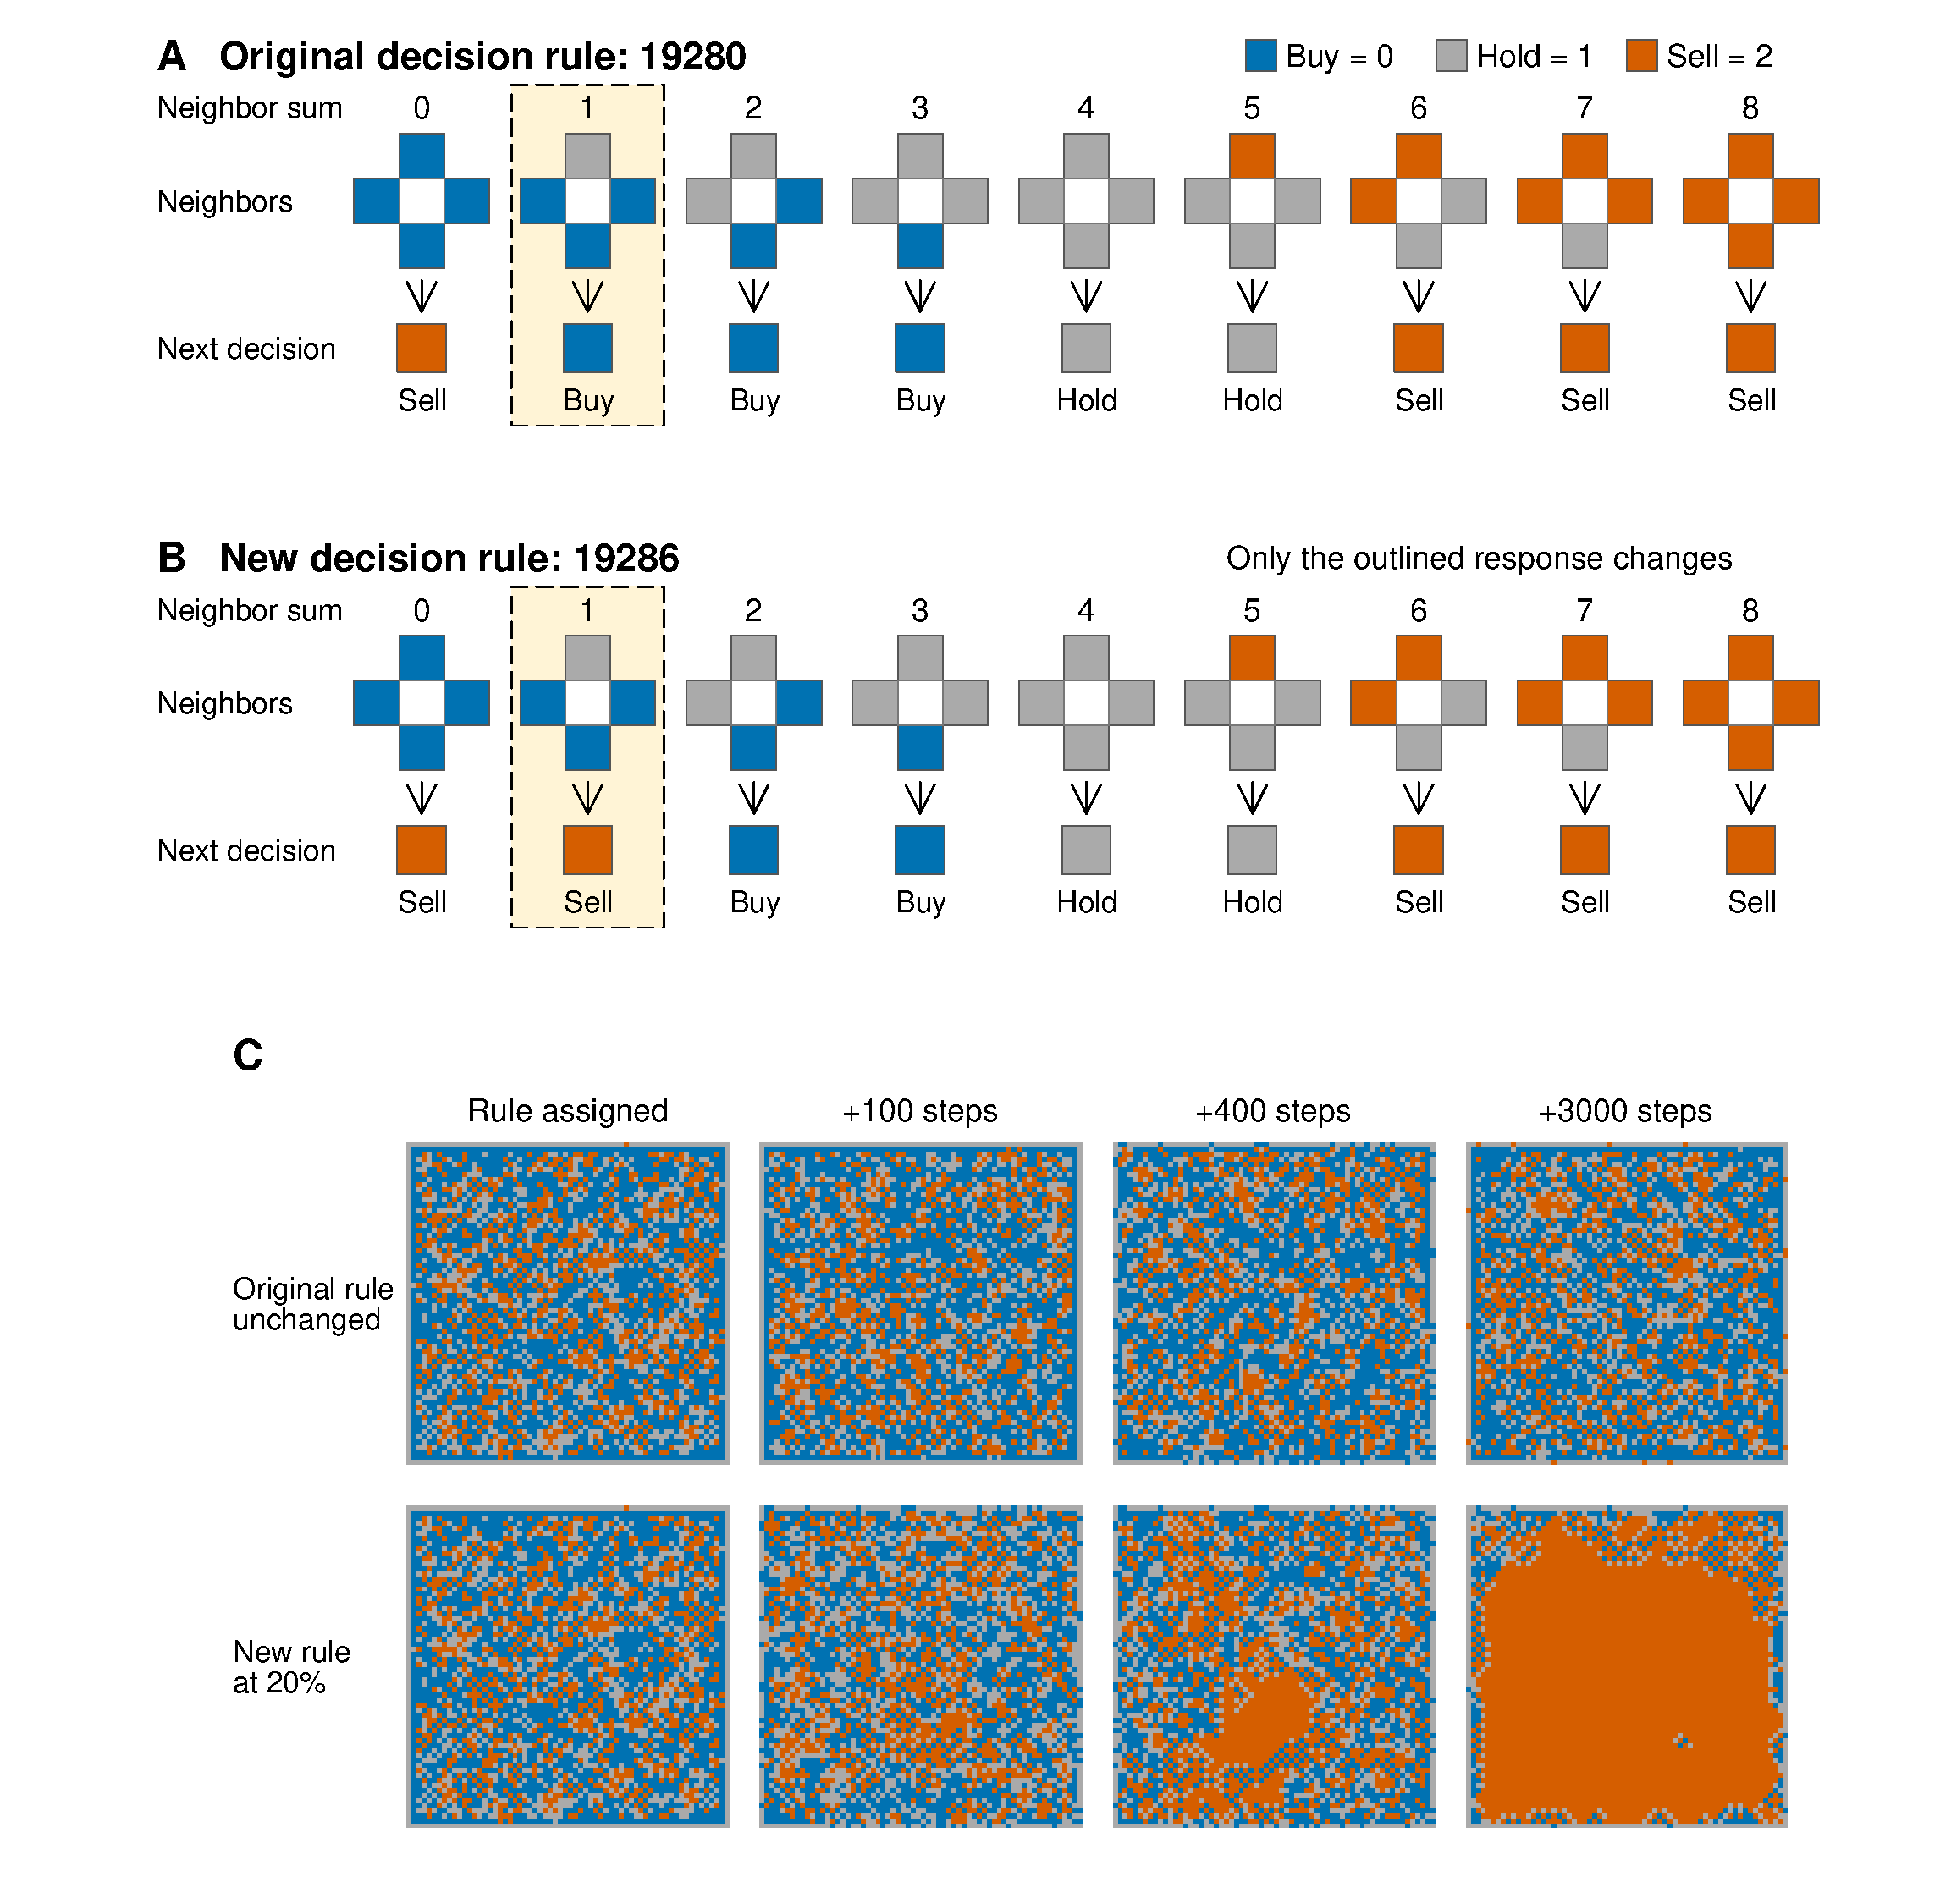
\includegraphics[width=0.95\linewidth]{figs/Fig1-RuleQuench.pdf}
\caption{The changed response and paired market decisions.
\textbf{(A)}~Baseline Rule~19280. \textbf{(B)}~Activated Rule~19286.
Each cross contains the four neighbors used to determine the next decision,
shown below its arrow. The hollow center is the trader being updated;
its current decision does not enter the lookup table. Blue, gray, and
orange denote Buy~(0), Hold~(1), and Sell~(2). One arrangement represents
each neighbor sum; every arrangement with that sum produces the same
response. The outlined column is the only rule change: three Buys and
one Hold produce Buy under the baseline and Sell under activation.
\textbf{(C)}~Paired $64\times64$ grids at activation and after 100,
400, and 3,000 steps. The upper row retains the baseline rule; the lower
assigns the new rule to 20\% of interior traders. Both paths share a
1,000-step baseline, $h=100$, and active technical traders. Starting
market 14 was selected from 50 by proximity to the
median paired difference in peak Sell fraction. Ensemble outcomes and
conditional onset times appear in Supplementary Table~\ref{tab:paired-switch}.}
\label{fig:rule-quench}
\end{minipage}
\end{center}

\clearpage

\begin{center}
\begin{minipage}{\linewidth}
\captionsetup{type=figure,hypcap=false}
\centering
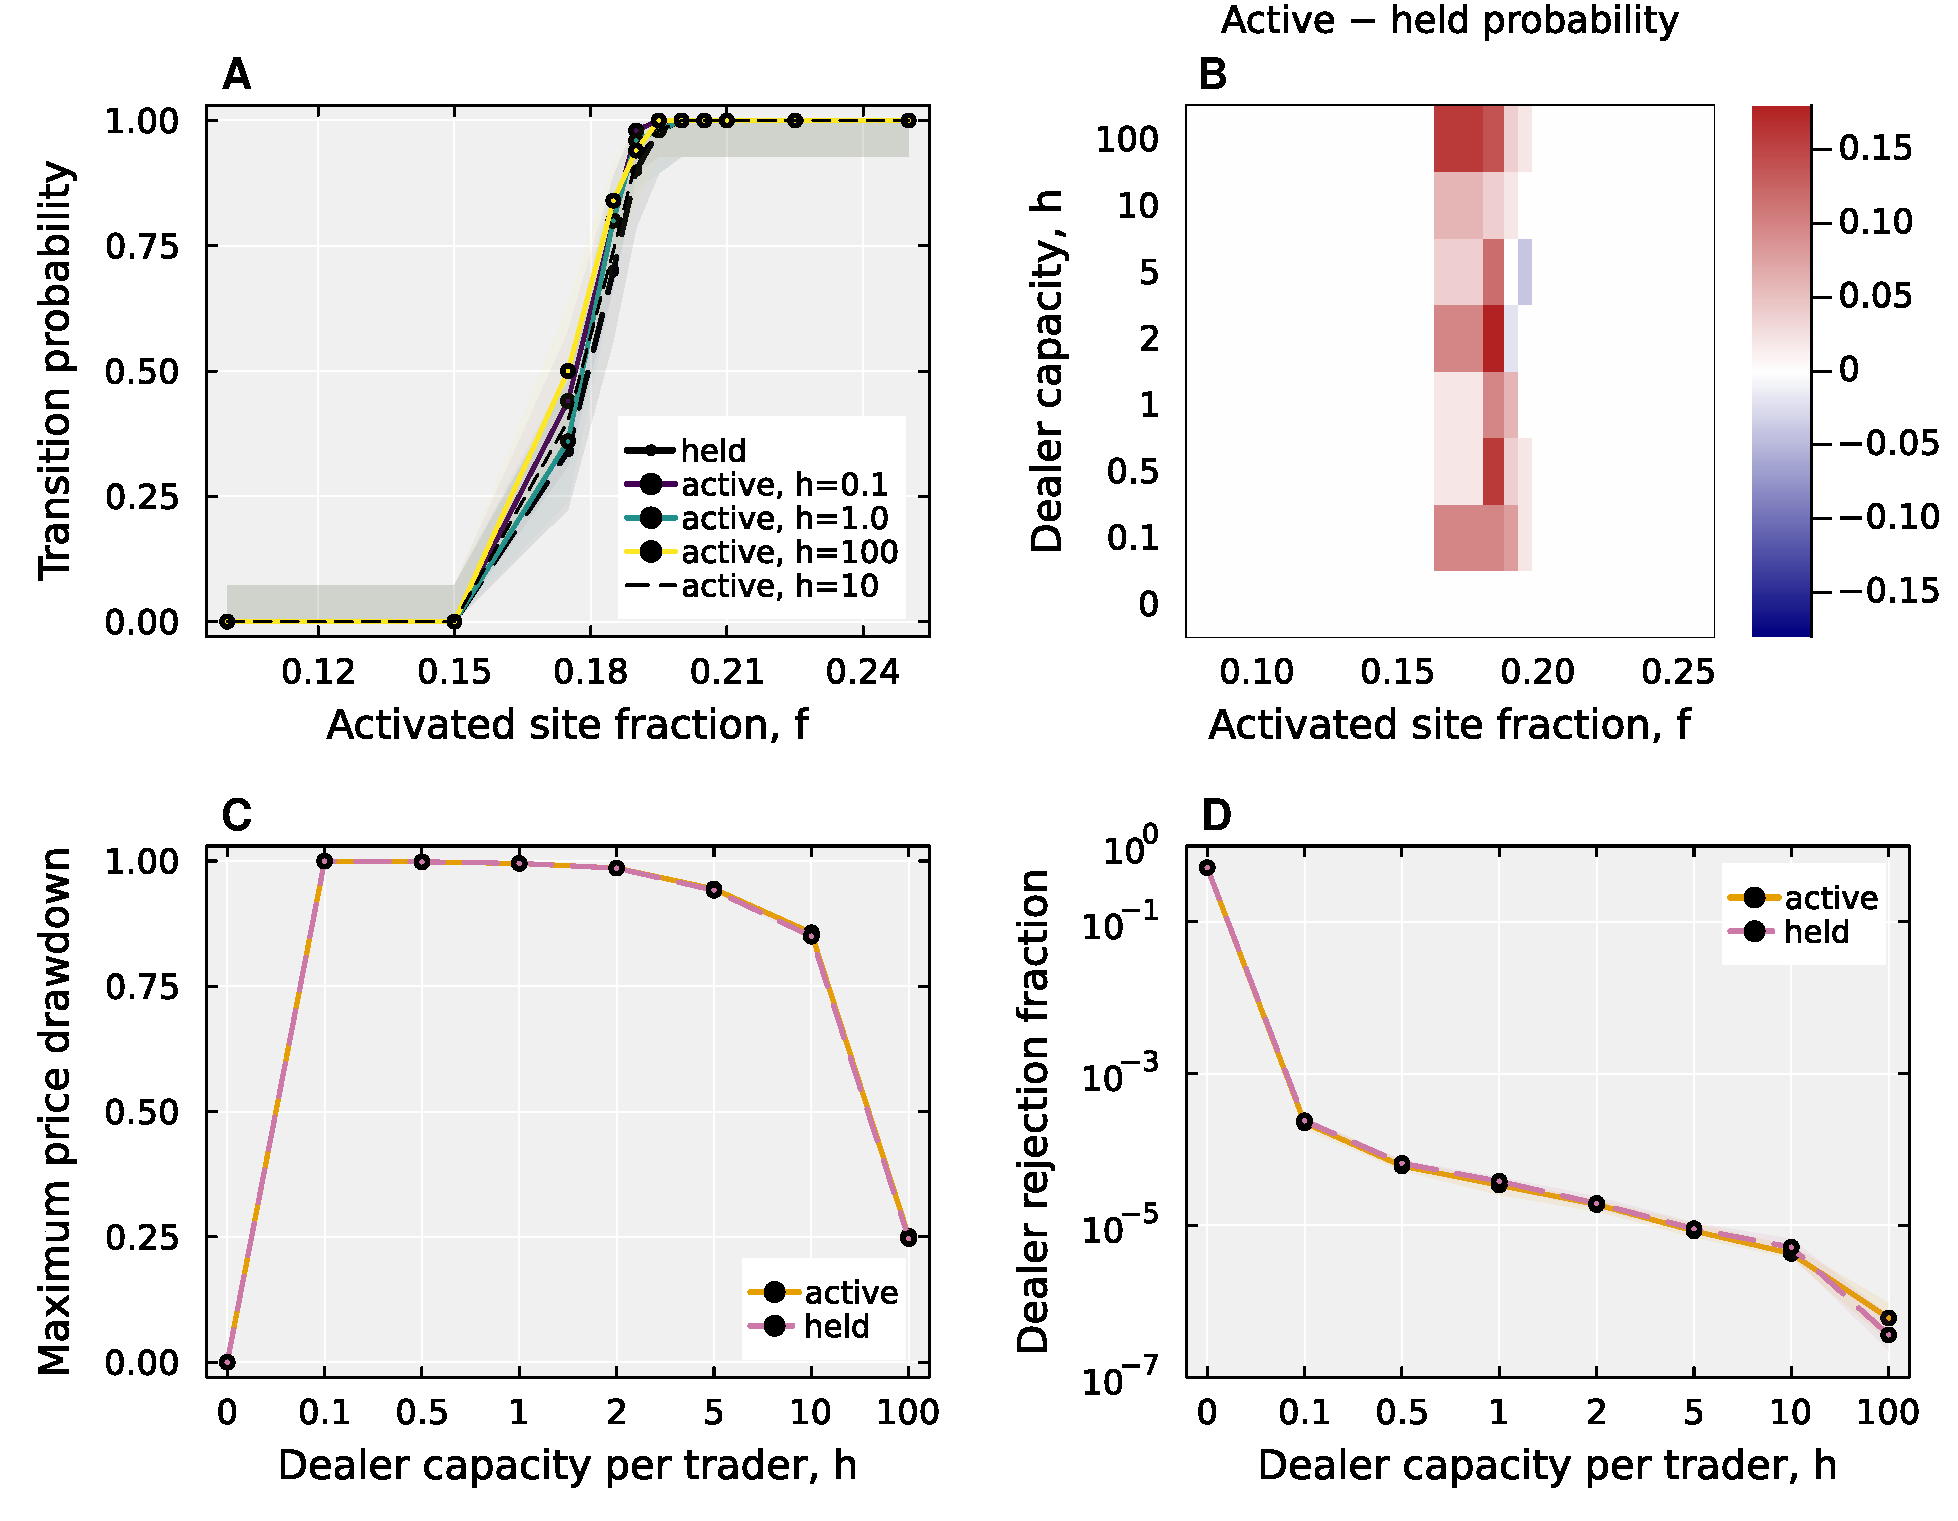
\includegraphics[width=0.97\linewidth]{figs/Fig2-ReservoirQuench.pdf}
\caption{Rule changes across dealer reserve depths over 3,000 post-switch steps.
\textbf{(A)}~Probability of an interior Sell majority with technical
traders held or active. Bands are 95\% Wilson intervals over 50 starting
markets. \textbf{(B)}~Active-minus-held majority probability at each
depth and target fraction. \textbf{(C)}~Median maximum drawdown at
$f=0.20$, with interquartile bands. \textbf{(D)}~Median fraction of
post-switch eligible orders rejected at $f=0.20$, on a logarithmic
axis with interquartile bands. Depth $h$ is initial dealer shares per trader and also determines
price sensitivity through the reserve curve. The $h=10$ dashed overlay
in A is a distinct finite-depth comparison; the deep arm is $h=100$.
At zero depth only opposing trader orders match and price stays fixed.
Panels C and D describe switched markets. Matched no-switch drawdowns
and paired differences appear in Supplementary Table~\ref{tab:paired-switch}.}
\label{fig:reservoir}
\end{minipage}
\end{center}

\clearpage

\begin{center}
\begin{minipage}{\linewidth}
\captionsetup{type=figure,hypcap=false}
\centering
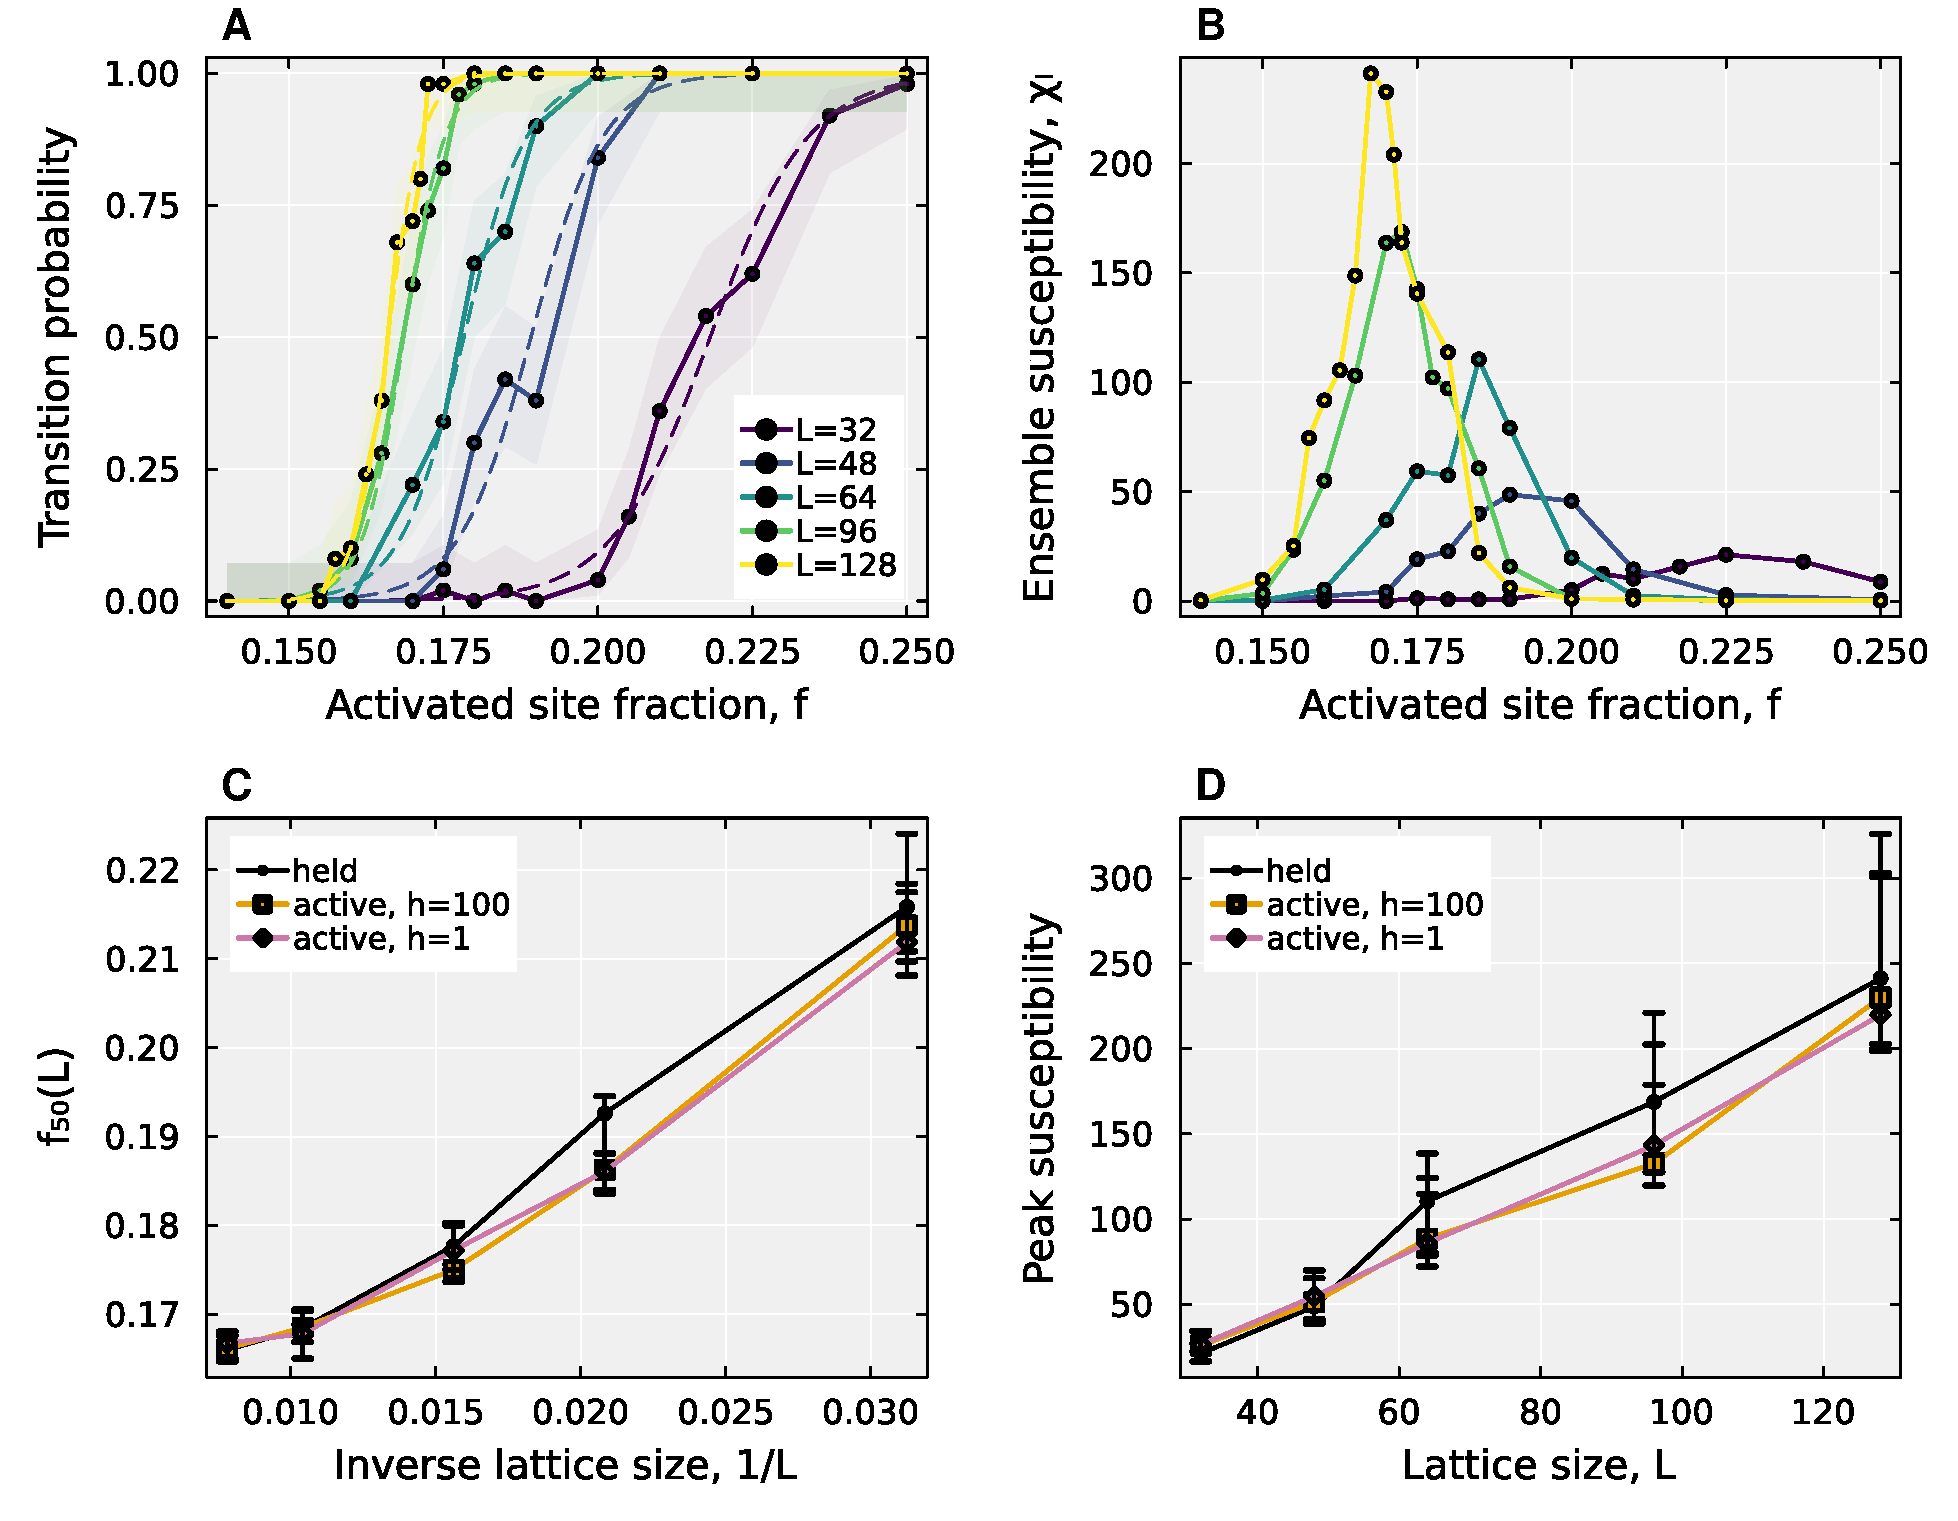
\includegraphics[width=0.97\linewidth]{figs/Fig3-FiniteSizeQuench.pdf}
\caption{Market size and the formation of a Sell majority
over 50 starting markets and 3,000 post-switch steps. \textbf{(A)}~Majority probability with technical
traders held, with 95\% Wilson bands. \textbf{(B)}~Susceptibility with
technical traders held: the variance across markets of the final
500-step mean Sell fraction, multiplied by the number of interior traders.
\textbf{(C)}~Interpolated fraction $f_{50}(L)$ at which half the markets
reached a majority, against inverse grid size, for held traders at $h=100$ and active traders at
$h=1$ and $h=100$. \textbf{(D)}~Sampled maximum susceptibility versus
grid size. Error bars in C and D are 95\% whole-market bootstrap
intervals. Solid lines connect tested values; dashed curves in A are
logistic fits. No law for indefinitely large grids was fitted.}
\label{fig:finite-size}
\end{minipage}
\end{center}

\clearpage

\begin{center}
\begin{minipage}{\linewidth}
\captionsetup{type=figure,hypcap=false}
\centering
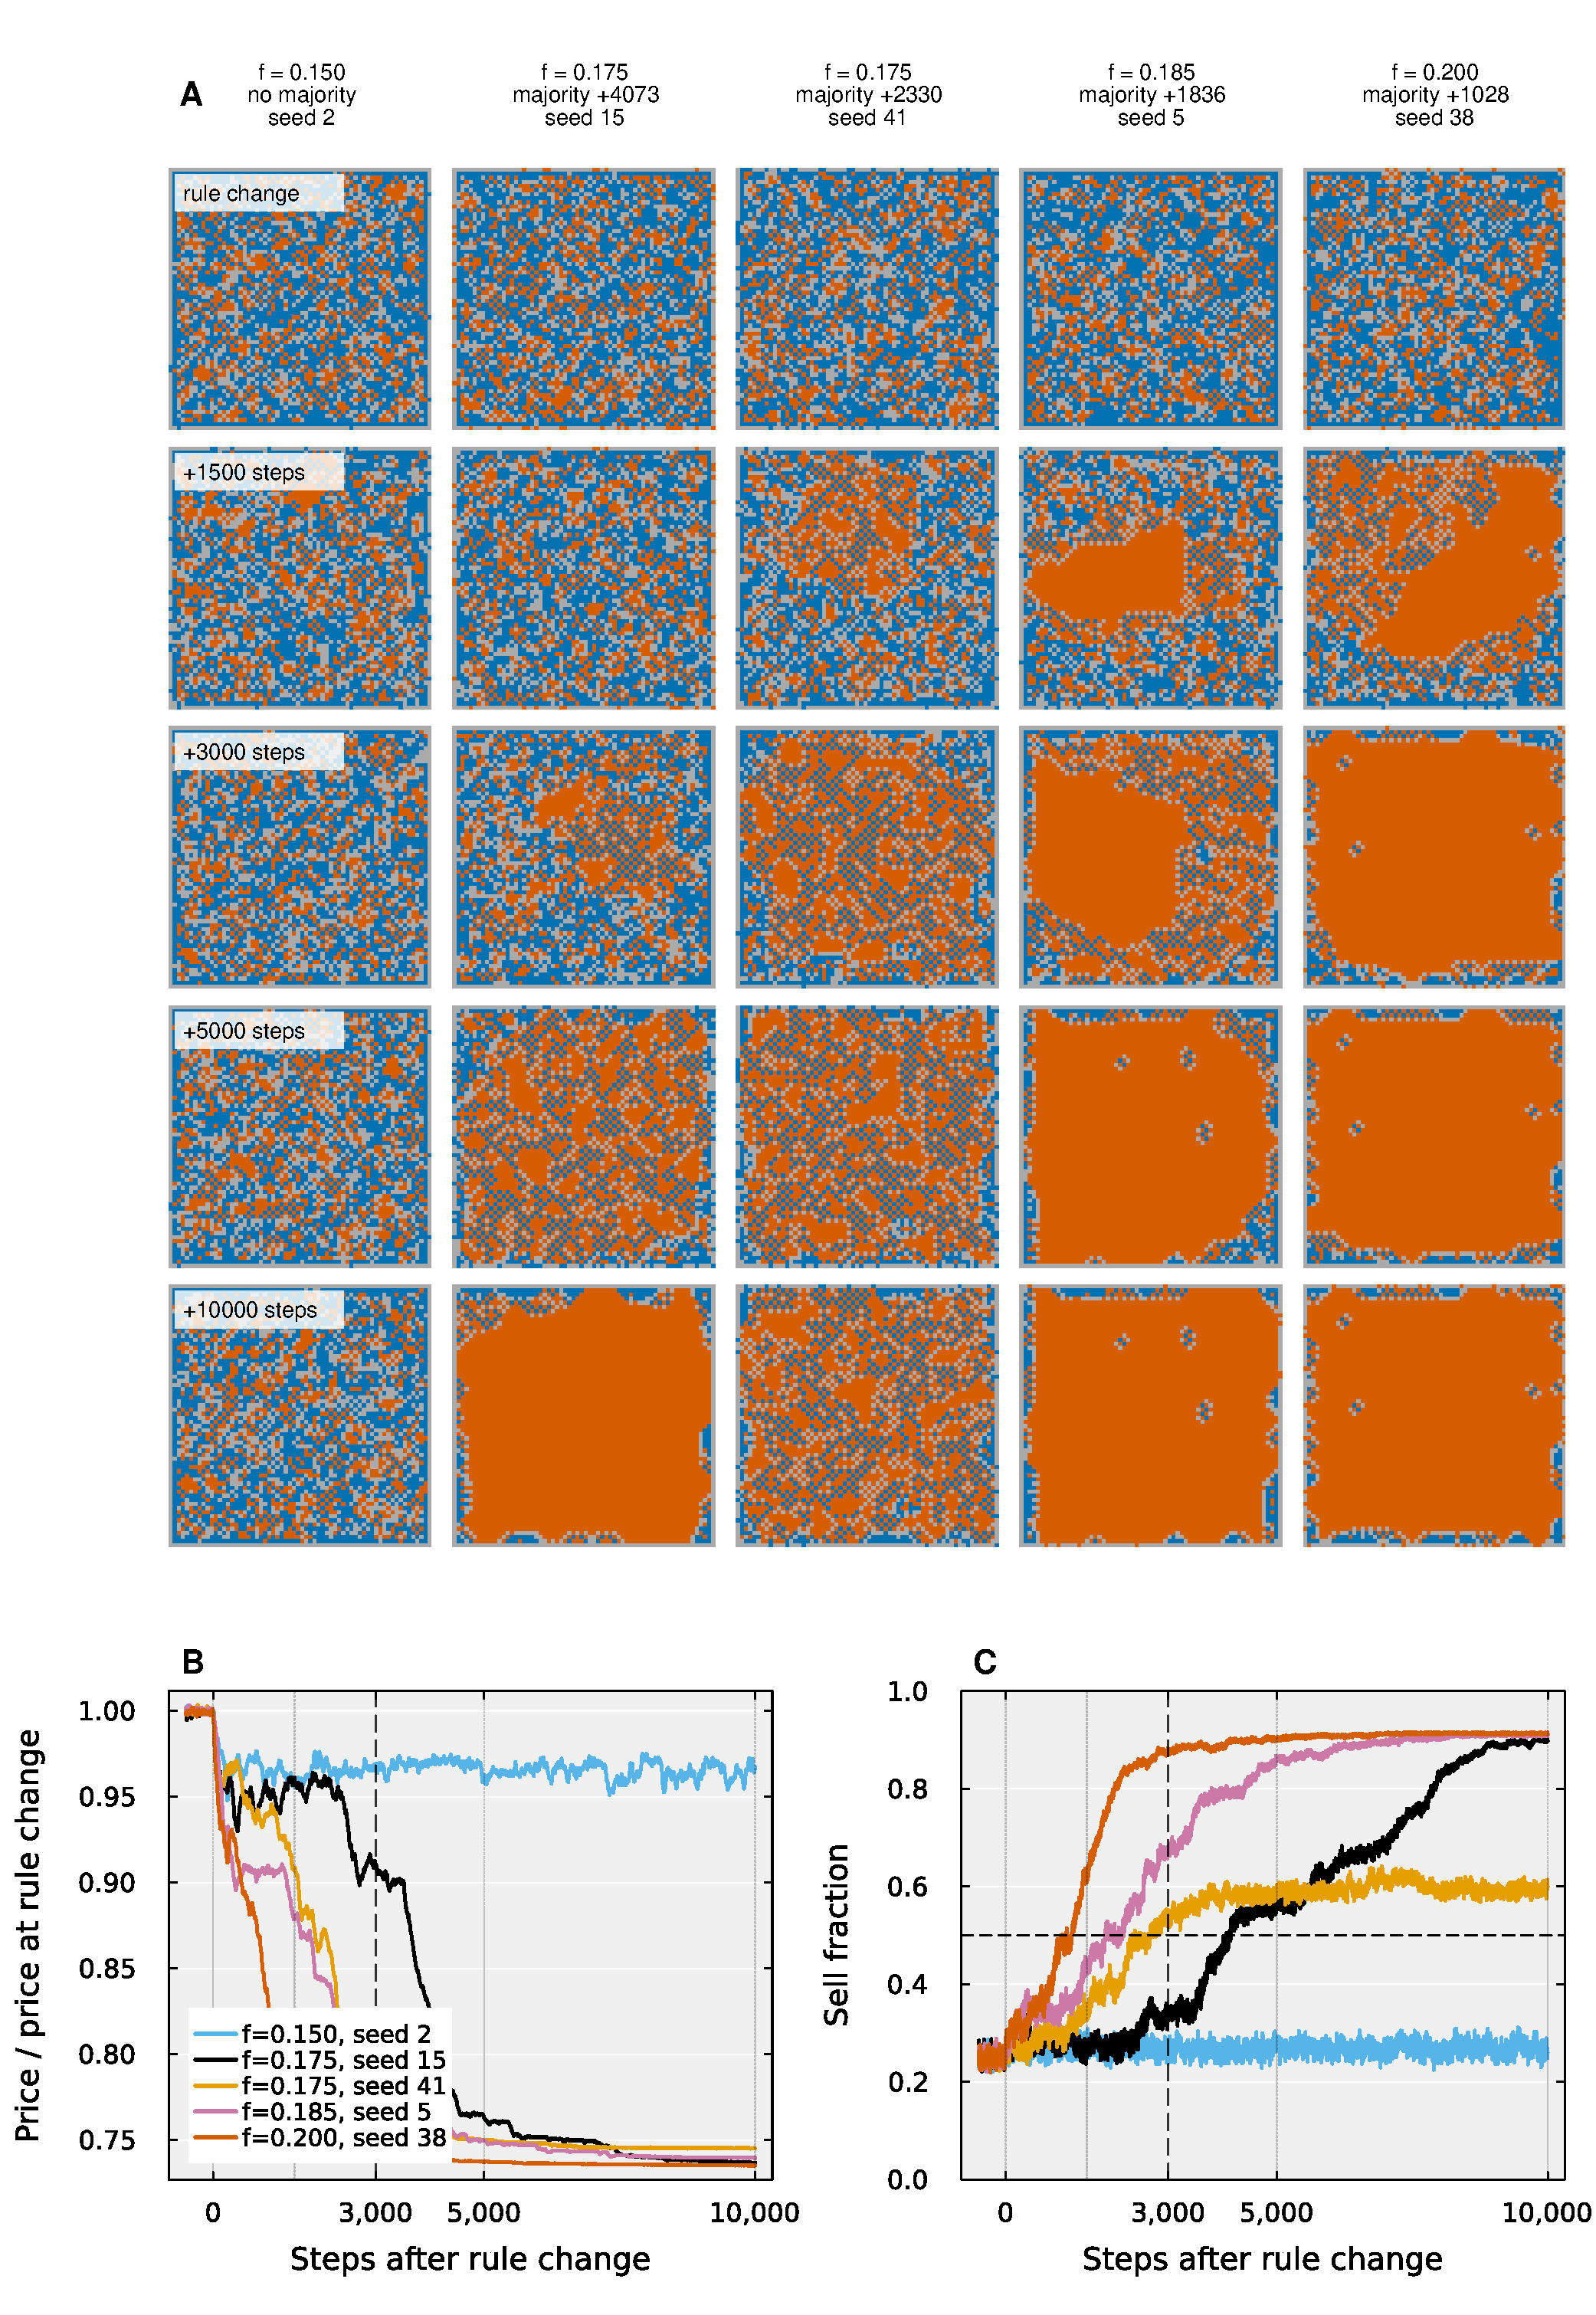
\includegraphics[width=0.90\linewidth]{figs/Fig4-DoseMarketPanels.pdf}
\caption{Longer histories of five numerically selected markets
with active technical traders and $h=100$. Blue, gray, and orange denote
Buy, Hold, and Sell. \textbf{(A)}~Grid decisions at activation and after
1,500, 3,000, 5,000, and 10,000 steps. Selection used the newly computed
3,000-step summaries before inspection of images. At that endpoint,
the first two markets had not reached a majority and the other three
had. Nonmajority examples were nearest their group's median final Sell
fraction; majority examples were nearest their group's median onset,
with seed breaking ties. Starting markets were 2, 15, 41, 5, and 38, from left
to right. The longer outcomes did not affect selection.
\textbf{(B)}~Marginal quote divided by its value at activation.
\textbf{(C)}~Interior Sell fraction, with one-half marked by a
horizontal line. The dark vertical dashed line marks the original
3,000-step endpoint; other guides mark the remaining snapshots.
Onsets and financial summaries appear in Supplementary
Table~\ref{tab:market-panel-horizons}.}
\label{fig:dose-panels}
\end{minipage}
\end{center}

\clearpage

\begin{center}
\begin{minipage}{\linewidth}
\captionsetup{type=figure,hypcap=false}
\centering
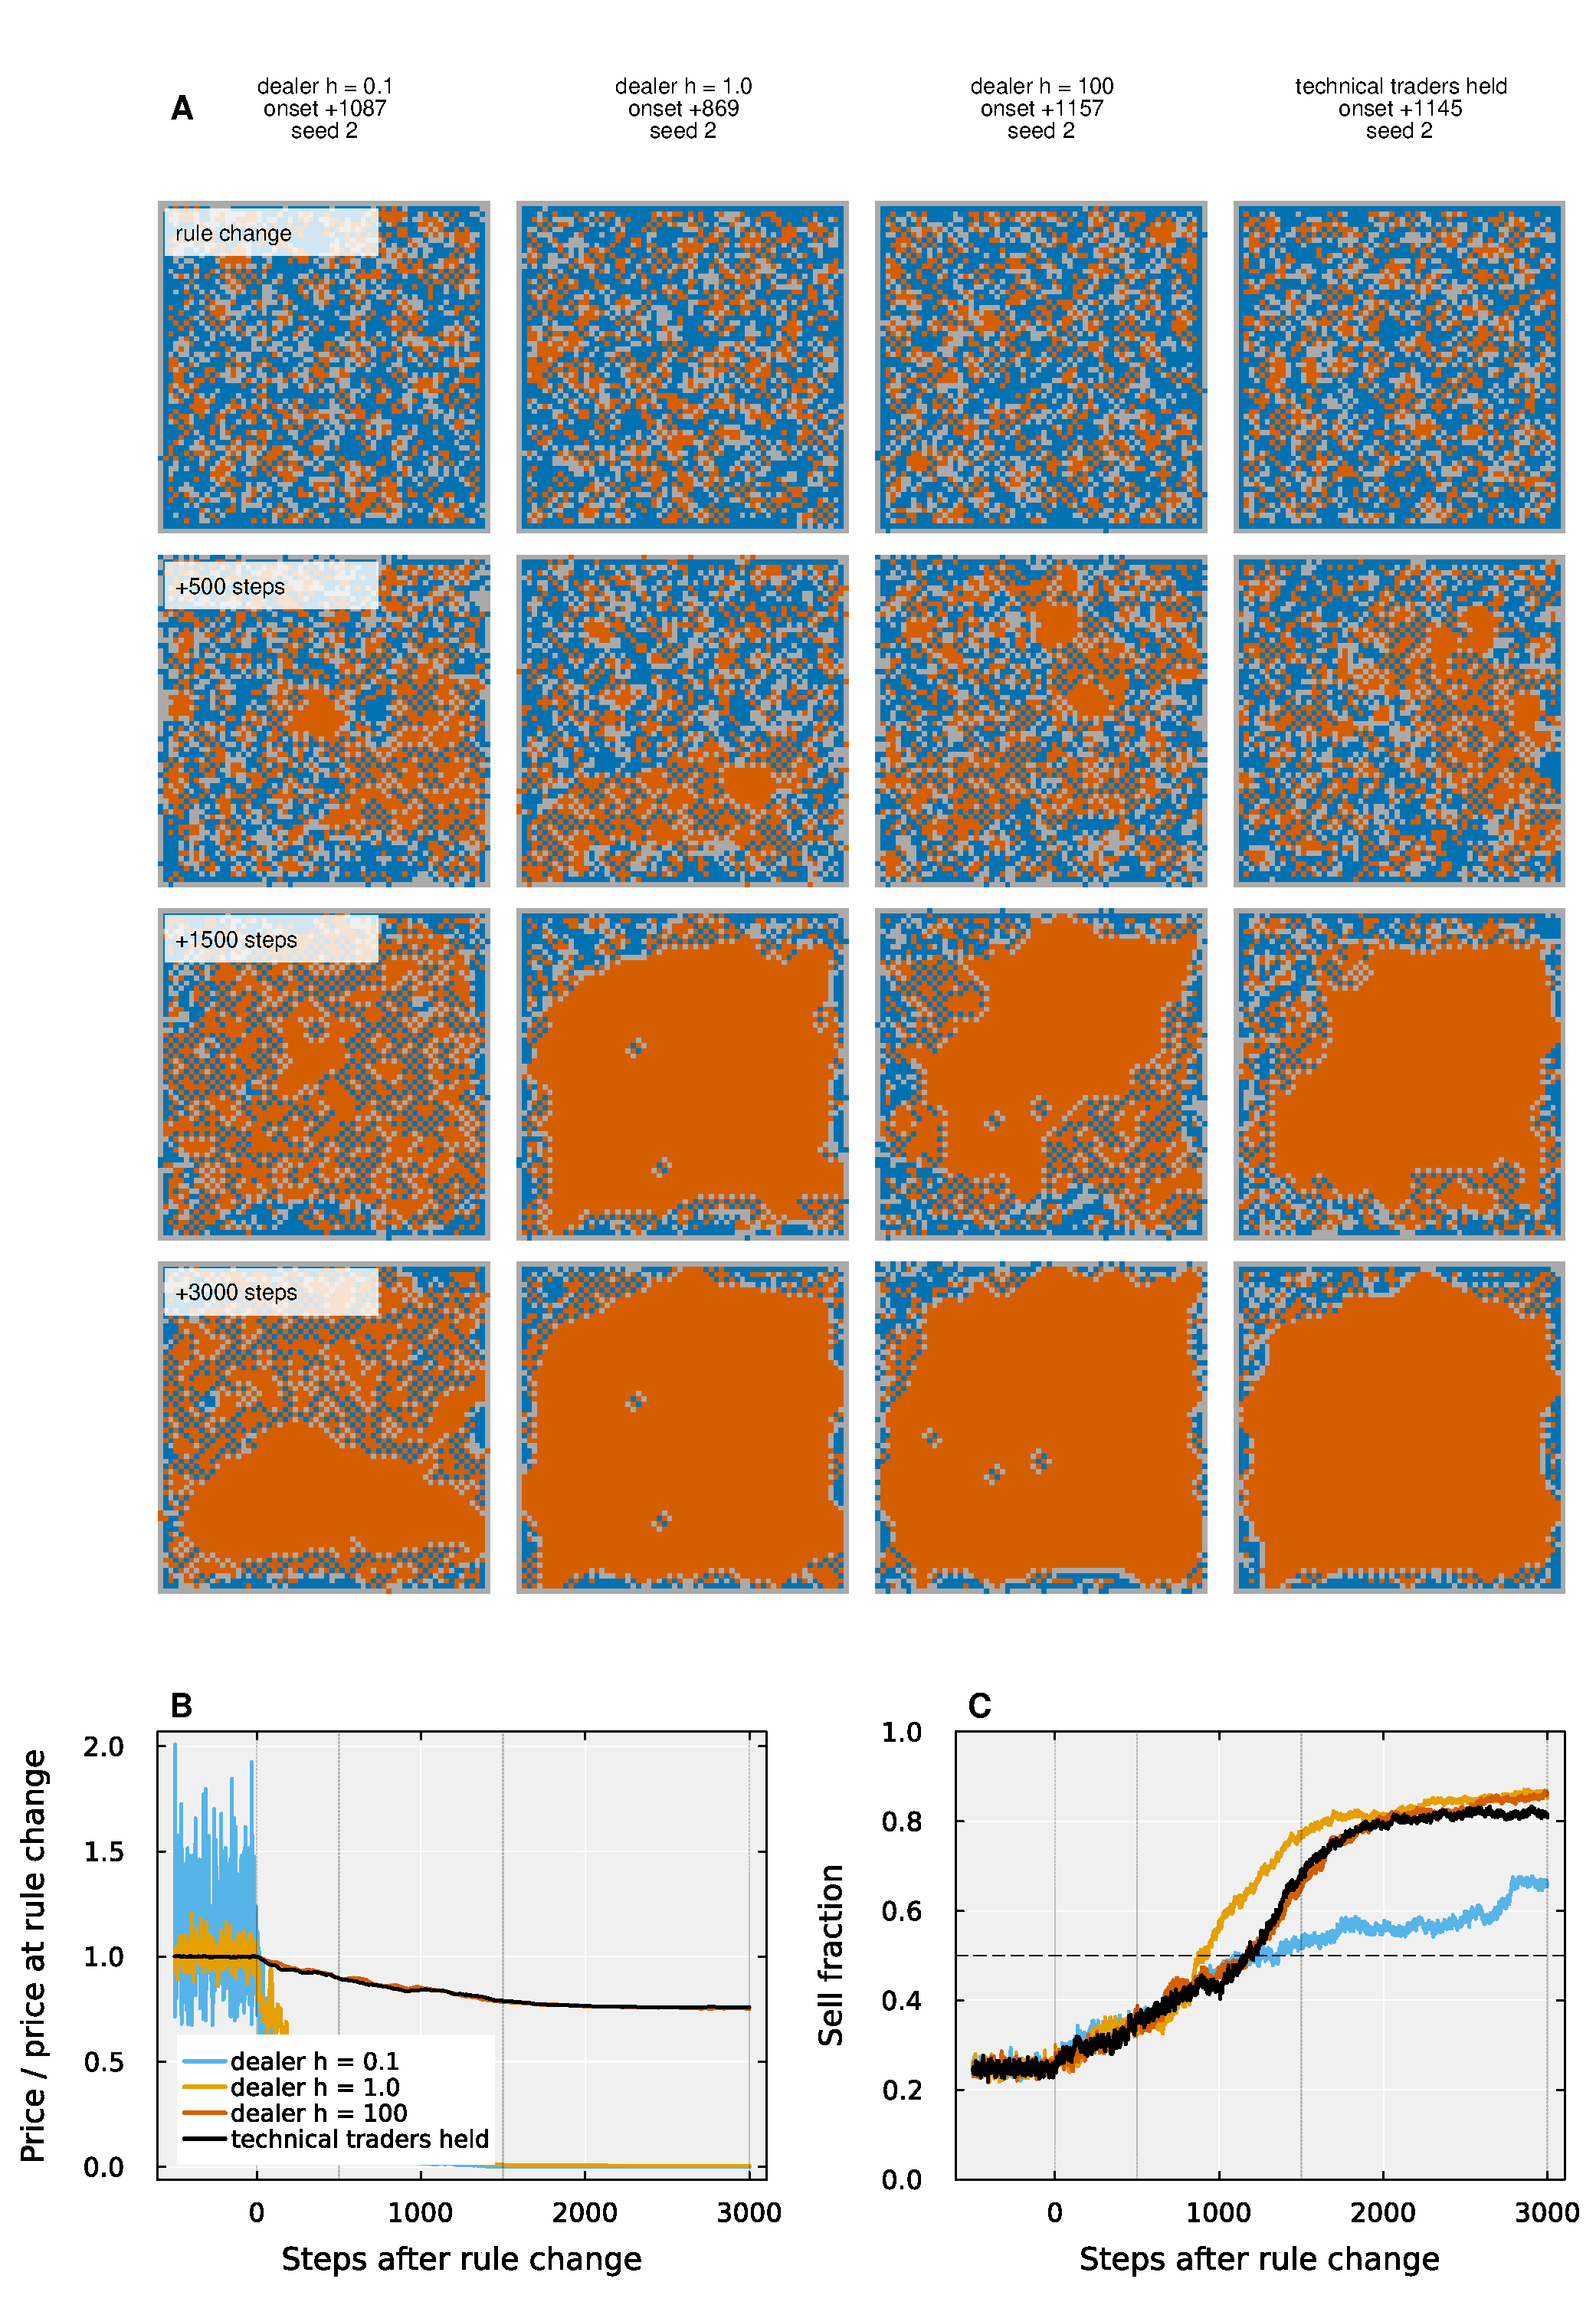
\includegraphics[width=0.92\linewidth]{figs/Fig5-DealerMarketPanels.pdf}
\caption{The same starting market at different dealer depths
with $f=0.20$. \textbf{(A)}~Grid decisions at activation and after
500, 1,500, and 3,000 steps. The first three columns have active technical
traders at $h=0.1$, $1$, and $100$; the last holds the technical traders
at $h=100$. Starting market 2 was selected among
markets reaching a majority at all three active depths by minimizing
the summed distance from their depth-specific median onsets, with seed
breaking ties. \textbf{(B)}~Marginal quote relative to activation.
\textbf{(C)}~Interior Sell fraction. The held condition prevents price
feedback into decisions while retaining full trading and price
calculations. The selected paths illustrate the same initialization
across conditions; ensemble probabilities and drawdowns appear in
Fig.~\ref{fig:reservoir}.}
\label{fig:dealer-panels}
\end{minipage}
\end{center}

\clearpage

\begin{center}
\begin{minipage}{\linewidth}
\captionsetup{type=figure,hypcap=false}
\centering
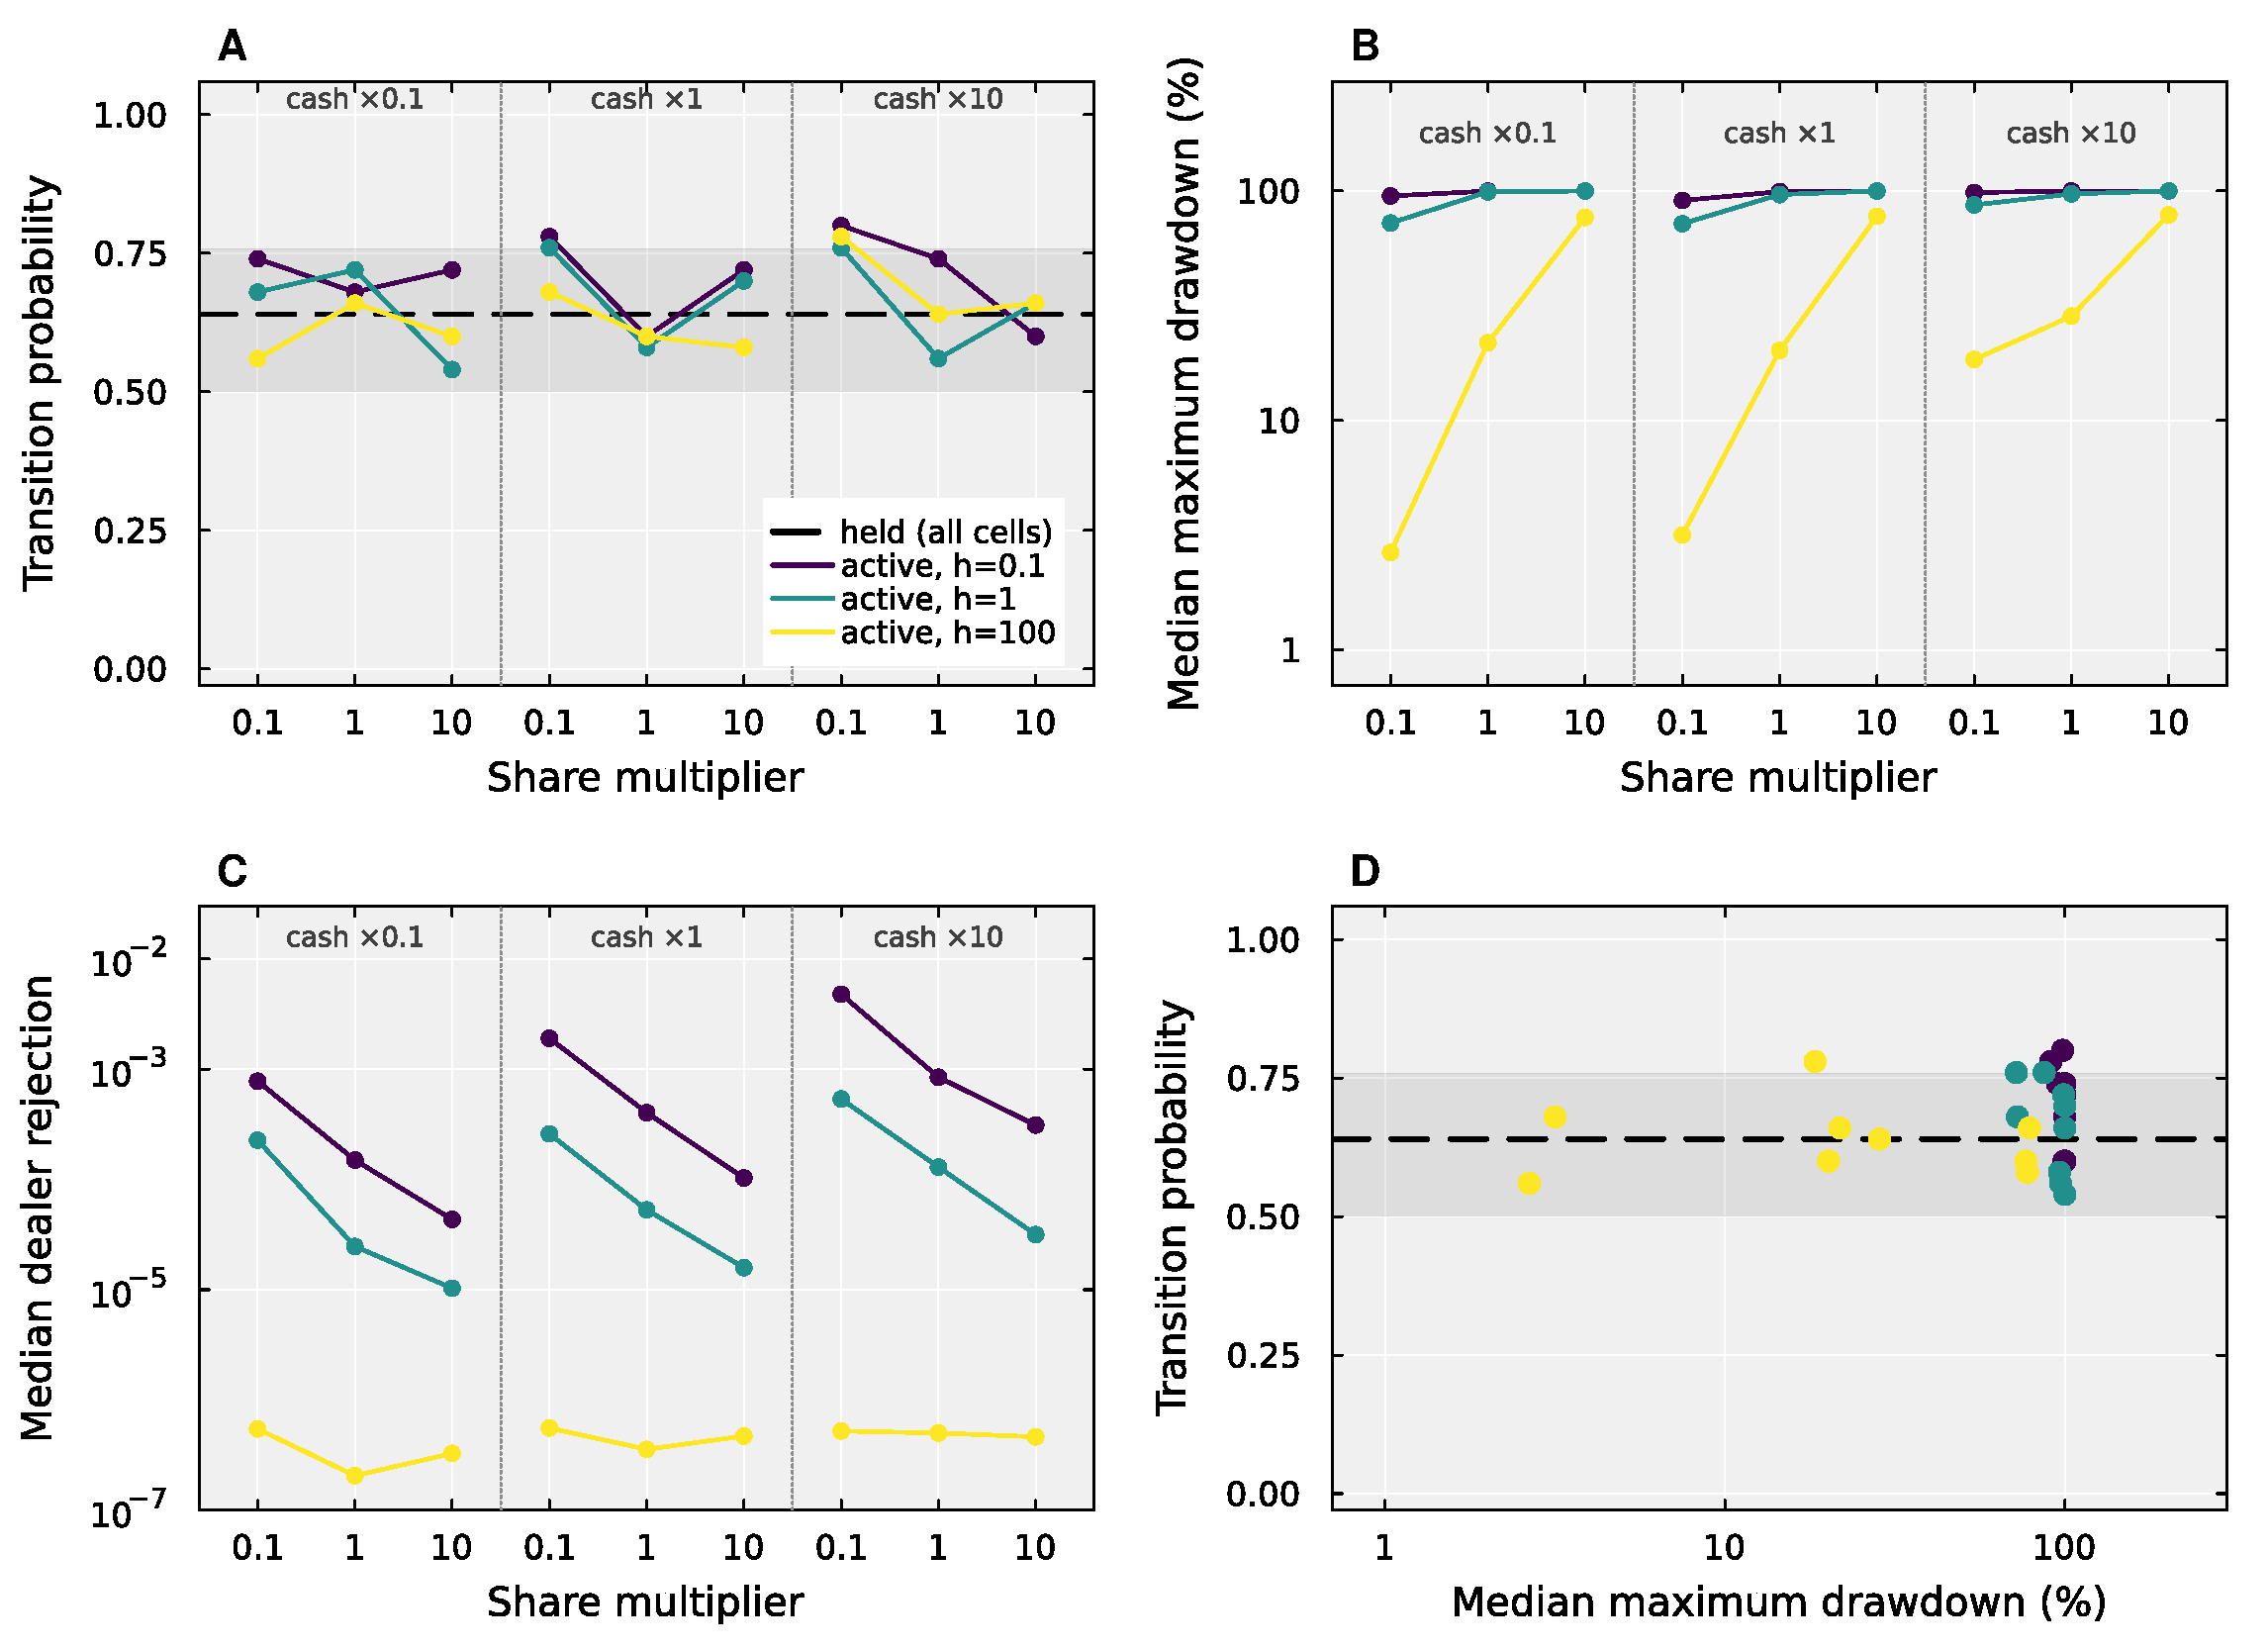
\includegraphics[width=0.99\linewidth]{figs/Fig6-BalanceSheetQuench.pdf}
\caption{Changing trader cash and shares at the rule switch,
with active technical traders, $f=0.18$, and 50 starting markets over 3,000 post-switch steps.
In A--C, the nine resource combinations are grouped by cash multiplier,
with share multiplier on the axis and a series for each dealer depth.
\textbf{(A)}~Majority probability. The dashed line and band give the
held-condition probability and its 95\% Wilson interval, identical
across financial conditions. \textbf{(B)}~Median maximum drawdown on a
logarithmic axis.
\textbf{(C)}~Median fraction of post-switch eligible orders rejected,
on a logarithmic axis.
\textbf{(D)}~Majority probability against median drawdown for all
27 active combinations, with the held reference repeated. The drawdown
axis follows B. Probability axes cover the full possible range;
all displayed drawdowns and rejection medians are strictly positive.}
\label{fig:balance-sheet}
\end{minipage}
\end{center}


\clearpage
\appendix

% appendix.tex -- Supplementary methods and validation
\section{Supplementary methods and validation}
\label{app:supplement}
\setcounter{algorithm}{0}
\renewcommand{\thealgorithm}{S\arabic{algorithm}}

\subsection{One complete simulation step}

The simulation separated a desired decision from its execution. Orders
used the decisions stored before the interior update, while technical
traders used the new marginal quote before the next interior decisions
were calculated. A resource shortage could therefore stop an order
without changing the state seen by neighboring traders. The uniform
execution price depended on the net quantity supported by the entire
batch (Eqs.~\ref{eq:execution-price} and~\ref{eq:dealer-buy-excess}), and
differed from the marginal quote left after settlement
(Eq.~\ref{eq:price-update}). Executed counts specified the net transfer
and its normalized imbalance (Eqs.~\ref{eq:dealer-sell-excess}
and~\ref{eq:imbalance}), which changed the dealer reserves
(Eq.~\ref{eq:dealer-ledger}). The new quote then updated the reference
band (Eq.~\ref{eq:adaptive-band}).
Algorithms~\ref{alg:model-step} and~\ref{alg:dealer-clearing} specify this
ordering for the main persistent-rule experiments with adaptive bands
and no cost-basis restriction. The pulse, alternative-rule, and frozen-band
controls modify the corresponding updates as described in
Appendix~\ref{app:revision-controls}.

\begin{algorithm}[!ht]
\caption{One market step, $t-1\rightarrow t$, in simulation order.
Stored decisions generated orders. Clearing determined a common execution
price, and the settled dealer reserves set the new marginal quote.}
\label{alg:model-step}
\begin{algorithmic}[1]
\REQUIRE grid $X_{t-1}$; technical-trader decisions; trader books; dealer
$(W_{t-1},Q_{t-1})$; quote and band state $(P_{t-1},\mu_{t-1},\sigma_{t-1})$;
rule field $R_i$; parameters; seed
\ENSURE grid $X_t$; technical-trader decisions; settled books and dealer;
quote and band state $(P_t,\mu_t,\sigma_t)$; order counts
\IF{$t$ is the scheduled rule-switch step}
 \STATE $R_i\leftarrow19286$ at the preselected target sites
 \COMMENT{preserve current decisions and financial state}
\ENDIF
\IF{$t$ is a scheduled resource intervention}
 \FORALL{traders $i$}
  \STATE $w_i\leftarrow g_w w_i$; $q_i\leftarrow\operatorname{round}(g_q q_i)$
 \ENDFOR
\ENDIF
\STATE call Algorithm~\ref{alg:dealer-clearing} using the stored decisions
\STATE receive settled books, dealer, order counts, execution price $F_t$, and quote $P_t$
\STATE $\mu_t\leftarrow\mu_{t-1}+\alpha(P_t-\mu_{t-1})$
\STATE $\sigma_t\leftarrow\sigma_{t-1}+\alpha(|P_t-\mu_t|-\sigma_{t-1})$
\IF{technical traders are active}
 \FORALL{technical traders $i$}
  \STATE $e_i(t)\leftarrow0$ if $P_t<\mu_t-k_i\sigma_t$; $2$ if
  $P_t>\mu_t+k_i\sigma_t$; $1$ otherwise
 \ENDFOR
\ELSE
 \STATE $e_i(t)\leftarrow1$ for every technical trader $i$
\ENDIF
\STATE write $e_i(t)$ to the selected perimeter sites; leave other perimeter sites in Hold
\FORALL{interior traders $i$, simultaneously}
 \STATE $c_i\leftarrow\sum_{j\in\partial i}s_j$ using old interior and new technical-trader decisions
 \STATE $s_i(t)\leftarrow\mathcal{R}_{R_i}(c_i)$
\ENDFOR
\end{algorithmic}
\end{algorithm}

\begin{algorithm}[!ht]
\caption{Uniform-price reserve clearing without a cost-basis restriction.
The binary search found the greatest supported integer net purchase in
the direction of initial excess demand.}
\label{alg:dealer-clearing}
\begin{algorithmic}[1]
\REQUIRE desired unit buys and sells from stored decisions; trader books
$(w_i,q_i,\bar c_i)$; dealer $(W,Q)$; previous quote; seed and step
\ENSURE settled books and dealer; order counts; execution price and next quote
\IF{$h=0$}
 \STATE use the previous quote; match opposing affordable buys and supplied sells
 \STATE apply seeded priorities if needed; settle matched orders; keep the quote fixed
 \RETURN settled books and order counts
\ENDIF
\STATE define $F(x)=W/(Q-x)$ for integer $x$ satisfying $Q-x\geq1$
\STATE define $B(x)$ as desired buyers with $w_i\geq F(x)$ and $S(x)$ as desired sellers with $q_i\geq1$
\STATE $d\leftarrow\operatorname{sign}[B(0)-S(0)]$; $\ell\leftarrow0$
\STATE $u\leftarrow\min(B(0)-S(0),Q-1)$ if $d>0$, otherwise $S(0)-B(0)$
\WHILE{$\ell<u$}
 \STATE $k\leftarrow\lfloor(\ell+u+1)/2\rfloor$
 \IF{$d[B(dk)-S(dk)]\geq k$}
  \STATE $\ell\leftarrow k$
 \ELSE
  \STATE $u\leftarrow k-1$
 \ENDIF
\ENDWHILE
\STATE $x\leftarrow d\ell$; $F_t\leftarrow F(x)$
\STATE collect eligible sets $\mathcal{B}$ and $\mathcal{S}$ at $F_t$
\STATE $n^B\leftarrow\min(|\mathcal{B}|,|\mathcal{S}|+x)$; $n^S\leftarrow n^B-x$
\STATE suppression $\leftarrow$ desired counts minus eligible counts
\STATE rejection $\leftarrow$ eligible counts minus executed counts
\STATE rank any rationed side by $z(\mathrm{seed},t,i,\mathrm{side})$, breaking ties by identity
\FORALL{selected buyers $i$}
 \STATE $\bar c_i\leftarrow(\bar c_iq_i+F_t)/(q_i+1)$;
 $q_i\leftarrow q_i+1$; $w_i\leftarrow w_i-F_t$
\ENDFOR
\FORALL{selected sellers $i$}
 \STATE $q_i\leftarrow q_i-1$; $w_i\leftarrow w_i+F_t$
\ENDFOR
\STATE $Q'\leftarrow Q-x$; $W'\leftarrow WQ/Q'$; $P_t\leftarrow W'/Q'$
\RETURN settled books, dealer, counts, $F_t$, and $P_t$
\end{algorithmic}
\end{algorithm}

\FloatBarrier

\subsection{Rationing and paired reproducibility}

Each eligible order on a rationed side received a 64-bit score from a
SplitMix64 finalizer applied to the simulation seed, step, trader identity,
and order side. Sorting by score, then identity, made rationing reproducible
while allowing priority to change over time. Paired markets used the same
score for the same trader and step even after their eligible sets diverged.
Scoring consumed no draws from the generator used for initialization.
For paired rule changes, comparisons checked the pre-switch grid and Sell
history, technical-trader coordinates and multipliers, and price history
through the first post-switch quote. A pure rule switch preserved that
first quote because the stored decisions still generated the same orders.
A one-time Sell pulse and a resource intervention could change the first
batch and therefore were required to agree only before the intervention.
For held technical traders, resource comparisons also required identical
Sell histories and final grids across all cash and share multipliers.

\subsection{Conservation and limiting cases}

Let total trader cash and shares be the sums over all traders. Outside
scheduled resource interventions, their combination with dealer reserves
satisfied the conservation identities:
\begin{align*}
 \sum_i w_i(t)+W_t&=\sum_i w_i(0)+W_0,\\
 \sum_i q_i(t)+Q_t&=\sum_i q_i(0)+Q_0.
\end{align*}
The production wrapper checked these identities separately before and
after an intentional resource change. Share conservation was exact.
The allowed absolute cash discrepancy was the larger of $10^{-5}$ and
$10^{-11}$ times total cash at the beginning of the checked interval.
For positive depth, checks required a finite positive quote, nonnegative
trader resources, preservation of the reserve product to relative
$10^{-9}$, and agreement between the quote and reserve ratio.
The implementation evaluated new dealer cash as $WQ/Q'$ to limit
accumulated rounding error; the equivalent transfer was $F_tx_t$.
These checks ran after every newly completed simulation, before its
execution record was written.

Zero depth permitted only matched trader orders and kept price fixed.
Technical traders then remained in Hold under either feedback condition,
providing an exact comparison between active and held interior decisions.
At positive depth, tests checked settlement at the selected price,
affordability after clearing, discrete rationing, and isolated round
trips that restored dealer inventory and cash. They also covered delayed
activation, preservation of a common prehistory, and the held-decision
invariance across financial interventions. An independent implementation
of the held decision update served as a test oracle. Every production
condition, including held decisions, was nevertheless rerun with the full
financial simulator. Finite depths were distinct model conditions: no
finite-depth path was assumed to equal an unlimited dealer.

\subsection{Simulation design and reproducibility}

The clean rebuild began with an empty data and figure tree and a frozen
copy of the corrected simulator, drivers, parameter manifest, and analysis
code. No earlier simulation output or checkpoint was imported. Completed
simulations wrote an execution ledger, while phase manifests and source
hashes constrained any resumption to outputs created within this rebuild.
All retained experiments were rerun, including held conditions whose
decisions could be predicted without calculating finances. Seeds were
retained to reproduce the planned starting markets; this was a complete
recomputation under the corrected model, not an independent sample of
starting markets. The corrected model replaced settlement at a standing
quote followed by a separate exponential price update. That earlier
mechanism admitted profitable isolated round trips, and its financial
outputs did not enter this manuscript. Reserve clearing changed both
settlement and price formation, so differences from the earlier model
cannot be attributed to one parameter alone.

The four main campaigns comprised 30,550 simulations over 50 starting
markets per condition and 3,000 post-switch steps
(Supplementary Table~\ref{tab:campaigns}). The selected paired-switch
campaign used $L=64$, $h=100$, and active technical traders at fractions
0.10, 0.15, 0.20, and 0.25. Dealer comparisons used fractions 0.10, 0.15,
0.175, 0.185, 0.190, 0.195, 0.200, 0.205, 0.210, 0.225, and 0.250 at
$h=0,0.1,0.5,1,2,5,10,100$ with technical traders active and held.
A newly simulated no-switch path was shared across fractions within
each depth, feedback condition, and starting market, avoiding duplicates
within the same campaign. The size campaign used $L=32,48,64,96,128$ at
fractions 0.140, 0.150, 0.160, 0.170, 0.175, 0.180, 0.185, 0.190,
0.200, 0.210, 0.225, and 0.250 before refinement. Its conditions were
held technical traders at $h=100$ and active technical traders at
$h=1$ and $h=100$. The cash and share campaign crossed independent
multipliers 0.1, 1, and 10 with fractions 0.170, 0.175, 0.180, and
0.185, depths 0.1, 1, and 100, and both feedback conditions. Dealer
resources increased with the trader count; no size series with fixed
absolute dealer resources was included.

The supplementary controls retained these starting-market conventions
while varying the intervention, reserve depth, band adaptation, or
observation window. Their fixed design preceded this clean rebuild;
adaptive refinement and example selection followed the numerical rules
specified above. We used Julia 1.12.7 with the repository environment
manifest, twelve simulation threads, and one garbage-collection thread.
A seeded Xoshiro generator supplied setup draws~\cite{blackman2021scrambled}.
Checkpointed drivers wrote atomic records and reconstructed a deterministic
row order. A recorded scheduling-only revision assigned supplementary jobs
to available workers individually. Validation against serial execution
and the original schedule reproduced complete market histories exactly;
the simulation equations, parameters, and analysis were unchanged. Python performed the bootstrap analysis and generated tables
from the new summaries. The accompanying repository snapshot contains source hashes, parameter
manifests, execution records, package versions, and derived outputs.
The project repository is
\url{https://github.com/varnerlab/Wolfram-markets-abm-paper}.
The repository retains earlier implementations and outputs as a record
of model development, outside the rebuild's permitted data inputs.

The example trajectories used newly computed 3,000-step summaries to
select typical markets before inspecting their images. We reran the five
selected conditions and all 50 starting markets at $f=0.150$ for 10,000
post-switch steps, each with a matched no-switch path
(Fig.~\ref{fig:dose-panels}; Supplementary Table~\ref{tab:market-panel-horizons}).
Selection was not repeated using the longer histories. Comparisons at the
original endpoint checked reproduction of the new short-run summaries;
additional figure reruns checked full histories and final grids for the
selected cases. The longer runs extended observations of the same
starting markets and did not supply independent replications. Majority
onset began with the first updated state after activation, and all
reported execution counts and rejection fractions used post-switch
steps. Keeping these measurement windows common avoided mixing baseline
trading into one campaign's financial summaries but not another's.


The completed rebuild was checked against its fixed parameter manifest and
its execution ledger. All fixed conditions were present, and the new size
and horizon campaigns with technical traders held agreed for 1,800 overlapping starting-market
and fraction combinations. Across the main dealer, size, and resource
campaign summaries, the largest absolute cash discrepancy was $3.40\times10^{-6}$,
and share discrepancies were zero. These numerical checks accompanied
the per-simulation reserve and conservation checks described above.

\subsection{Additional controls and sensitivity analyses}
\label{app:revision-controls}

The supplementary controls used the same initialization and baseline as
the main comparisons, with grid size $L=64$, dealer depth $h=100$, and 3,000 post-intervention
steps unless otherwise specified. Every switched run was compared
with a no-switch control. Held conditions calculated full
financial histories as well as decisions. A Sell pulse wrote Sell
at the selected interior traders immediately before the first post-baseline orders,
while retaining the baseline rule for later updates. Traders already in
Sell were unchanged. A persistent intervention instead changed the
selected rule without overwriting decisions, so its first price remained
identical to the no-switch price. These paired interventions compared
the same fractions and starting markets under both technical-trader
conditions (Supplementary Table~\ref{tab:revision-pulse}). The rule
screen tested all eighteen ways of changing one response in the
baseline lookup table, using twenty starting markets per condition
and three fractions. Each screen entry was descriptive rather
than a separate confirmatory hypothesis test
(Supplementary Table~\ref{tab:revision-rules}).

The band control froze the recent-departure scale at its value immediately
before the rule switch, while each technical trader retained its multiplier
and the reference price continued to update. Adaptive and frozen runs
shared their complete pre-switch histories. The frozen widths could
therefore differ across dealer depths and starting markets. At fraction $f=0.175$,
the estimated majority-probability difference between dealer depths $h=0.1$ and
$h=100$ was -0.06 with adaptive widths and -0.26 with
frozen widths. Subtracting those two differences gave
0.20, with a 95\% whole-market bootstrap interval of
[-0.08, 0.50] (Supplementary Table~\ref{tab:revision-band}).
This comparison changed width adaptation while retaining the response
to departures from a moving reference price. It therefore tested one
part of the price feedback rather than removing technical trading.

Additional comparisons used dealer depths $h=40,100,400$ at fraction $f=0.20$ with
active technical traders (Supplementary Table~\ref{tab:revision-impact}).
For the constant-product dealer, differentiating log price with respect to
normalized net trader purchases at initialization gives $2N_{\rm tr}/H$,
approximately $2/h$. The chosen depths therefore spanned initial slopes
0.05, 0.02, and 0.005. No independent exponential impact coefficient
was varied: changing depth also changed dealer funding. These
comparisons replaced an impact-coefficient sweep belonging to the
superseded standing-quote model. They measured sensitivity within the
corrected mechanism and did not hold available reserves fixed while
changing price sensitivity. Neither the quoted price nor the length of a step was
calibrated to an observed market.

The horizon campaign used fifty starting markets at fractions
0.140, 0.145, through 0.250, extending to 0.300 for grid size $L=32$ to bracket
short-horizon responses. Held technical traders prevented financial
feedback throughout. Endpoint comparisons used the original 3,000 steps
and size-dependent observation periods $3000(L/64)^z$ for $z=1,2$, alongside longer
observations. Majority criteria of 0.4, 0.5, and 0.6 were extracted
from each history. Interpolation and bootstrap intervals were calculated
separately for every size, horizon, and criterion
(Supplementary Table~\ref{tab:revision-horizons}). The no-switch
extension followed ten starting markets per technical-trader condition for
100,000 additional steps. The observed outcomes were active technical traders: 0/10 majorities, 95\% Wilson interval [0.000, 0.278]; held technical traders: 0/10 majorities, 95\% Wilson interval [0.000, 0.278].
These extensions reused starting markets and did not constitute
independent replications. The observed frequencies of Sell majorities described
the stated interval without establishing behavior at indefinitely long
times.

We also characterized the shared pre-switch histories at dealer depth $h=100$ with
active technical traders. Across the fifty starting markets, mean
interior Sell fractions were 0.2494 over
steps 501--750 and 0.2504 over steps
751--1,000. In the latter interval, the median within-market log-return
standard deviation was 0.000323, and
median within-market first and ninety-ninth percentiles were
-0.000730 and
0.000729. The mean fraction of exactly
zero computed log returns was 0.007.
These summaries described the starting markets without establishing
stationarity or matching a calibrated empirical return distribution.
The no-switch controls separately measured post-switch baseline
financial variation across dealer depths
(Supplementary Table~\ref{tab:paired-switch}).

The refined finite-size analysis resampled entire starting markets across
fractions in 2,000 bootstrap replicates. The empirical estimate used the
first upward crossing and allowed local decreases in probability, while
the logistic fit imposed a smooth increasing response
(Supplementary Table~\ref{tab:revision-fits}). Each replicate reselected
the susceptibility maximum over the tested fractions. Consequently,
intervals included variation in which sampled fraction supplied that
maximum, but not interpolation bias, uncertainty from selecting the
refinement grid, or changes from observing for longer. The recorded
valid-bootstrap fraction identified samples in which the requested
crossings remained bracketed. No susceptibility exponent or
infinite-size limit was fitted.



\end{document}
